\documentclass{article}
% The ICLR style file lives next to the CoSpRo paper; this report reuses it.
\usepackage{../../paper/iclr2027_conference,times}
\iclrfinalcopy
\usepackage[T1]{fontenc}
\usepackage{amsmath,amssymb,booktabs,tabularx,microtype}
\usepackage{graphicx}
\usepackage{float}
\usepackage{xcolor}
\usepackage{hyperref}
\usepackage{url}
\hypersetup{hidelinks}
\usepackage[section]{placeins}
\usepackage{tikz}
\usetikzlibrary{arrows.meta,positioning,calc}
\setlength{\emergencystretch}{2em}

\definecolor{catc}{HTML}{2A78D6}
\definecolor{couchc}{HTML}{EB6834}
\definecolor{windowc}{HTML}{8A8F98}

\tikzset{
  box/.style={draw=black!75,rounded corners=1pt,align=center,font=\small,inner sep=4pt,fill=white},
  tbox/.style={box,fill=black!5},
  lbox/.style={box,fill=black!10},
  arr/.style={-{Stealth[length=2mm]},thick,draw=black!70},
  darr/.style={-{Stealth[length=2mm]},thick,dashed,draw=black!60},
}

% Toy scene in map-cell units (0..14, y upward): couch, window and cat.
\newcommand{\toyscene}{%
  \fill[couchc!45] (6,2) rectangle (13,7);
  \fill[windowc!35] (9,9) rectangle (13,13);
  \fill[catc!55] (5,7) ellipse (2 and 2.6);
}

\title{SCD: Spatial Concept Distillation\\for Spurious-Correlation Robustness\\in Self-Supervised Pretraining}
\author{}
\begin{document}
\maketitle
\lhead{}

\begin{abstract}
Self-supervised representations inherit the co-occurrences of their unlabeled training images: when cats appear mostly indoors, an encoder trained from scratch learns indoor scenes as evidence for cats and fails on cats outdoors. Methods that counter this usually assume which feature is spurious, such as the background or the easiest feature. We introduce Spatial Concept Distillation (SCD), which makes no such assumption and tells the encoder \emph{where} each named concept sits in an image. Before training, a frozen vision-language teacher (CLIP with a sparse concept decomposition) names the concepts of the training set and computes a dense map of every concept for every training image. During self-supervised pretraining, every location of the student's last feature map has to predict the concepts at its place in the view. At the level of whole images an object and its usual surroundings arrive together; at the level of locations they occupy different places, so the student needs a separate code for each. The prediction runs through a linear readout fitted on one half of the batch and scored on the other half, so memorizing individual images earns nothing and only concept codes shared across images lower the loss. No class label, group annotation or concept type enters pretraining and only the student encoder is kept for inference. We evaluate SCD against SimCLR and against our earlier relational method CoSpRo on three benchmarks of spurious correlations, with controls that separate the content of the maps, the role of concept names and the role of location.
\end{abstract}

\section{Introduction}
An image can contain several predictive factors. In Waterbirds the bird category correlates with the background of the training images; in MetaShift 88\% of the training cats sit indoors and 88\% of the dogs outdoors. A representation that encodes the object together with its usual surroundings fails on birds in an uncommon environment and on cats on a lawn. Worst-group evaluation makes these failures visible when the average accuracy hides them \citep{sagawa2020groupdro}. Self-supervised pretraining inherits the correlations of its unlabeled images: SimCLR rewards every feature that tells two images apart, the couch as much as the cat \citep{chen2020simclr} and the augmentations leave open which changes of the context should preserve the identity of the object.

Our goal is a visual encoder whose downstream predictions stay useful when object--context associations change. Pretraining may use no target labels, no group annotations and no knowledge of which concept is spurious, since that knowledge differs between datasets: the background in Waterbirds, gender in CelebA with hair colour as the target. Deep feature reweighting shows that a linear head retrained on a small group-balanced set recovers worst-group accuracy whenever the representation encodes the core feature apart from the spurious one \citep{kirichenko2023dfr}. The question is therefore how to make a self-supervised encoder carry the cat as a feature of its own.

Our previous method, CoSpRo, approached this question through pairs of images. It removed the subspace of a concept group from frozen CLIP embeddings, kept the image pairs that became similar and transferred the resulting graph to a SimCLR student through a relational loss. CoSpRo improved Waterbirds and stayed at the SimCLR level on MetaShift and Spur-CIFAR10. It also relied on a prior: that the spurious attribute is a context concept whose removal reveals a useful relation.

SCD rests on a different observation. At the level of whole images, cat and couch arrive together on most training images; a student that sees only whole-image targets can satisfy them with one fused ``cat-and-couch'' feature. At the level of locations, the cat and the couch occupy different places in \emph{every} image. A student that has to say ``cat here, couch there'' for every part of every view needs one code for the cat and another for the couch. Location separates what co-occurrence fuses and it does so for every concept alike, with no decision about which concept is spurious.

SCD turns the concepts of the training set into dense maps with a frozen CLIP model and asks every location of the student's last feature map to predict the concept values at its place in the view. A ridge regression fitted on one half of the batch scores the other half, so only concept directions shared across images lower the loss. During inference only the trained encoder and the downstream classifier remain.

Our contributions are:
\begin{itemize}
\item a prior-free spatial concept loss for self-supervised pretraining, built from named concepts that a frozen vision-language model locates on the training images;
\item a cross-fitted regression readout that makes the loss reward concept codes shared across images and gives memorization of single images no reward;
\item a controlled study on three datasets, with controls that separate the concept content of the maps (shuffled maps), named concepts against generic dense CLIP information (principal-component maps) and the role of location (image-level concept regression), a matched comparison with CoSpRo and a post-hoc audit of which concepts the student carries to unseen images.
\end{itemize}

\section{Related Work}
\paragraph{Dense and region-level self-supervised learning.}
SimCLR contrasts two views of an image against the other images in the batch \citep{chen2020simclr} and pools the feature map before its projection head. DenseCL adds a contrastive loss between matched locations of the two views \citep{wang2021densecl} and PixPro asks locations that cover the same image pixels to agree \citep{xie2021pixpro}. DetCon pools the feature map inside unsupervised masks and contrasts the pooled regions across views \citep{henaff2021detcon}. These methods supervise locations with the student's own features or with unnamed segments. SCD supervises every location with named concept values from a frozen teacher and keeps the SimCLR objective unchanged.

\paragraph{Dense concepts from vision-language models.}
CLIP supplies a shared image--text space \citep{radford2021clip}. Its patch tokens carry little local information in the last block, where every patch attends to the same few global tokens \citep{zhou2022maskclip,wang2024sclip,darcet2024registers}. MaskCLIP aligns patch tokens with text once the last attention pooling is bypassed \citep{zhou2022maskclip}; SCLIP replaces the query--key attention by a correlative self-attention \citep{wang2024sclip}; ClearCLIP removes the residual and feed-forward branches of the last block and uses query--query attention \citep{lan2024clearclip}. All three need no training. SCD uses the ClearCLIP construction offline on the training images only and reads images through overlapping windows, as SCLIP and ClearCLIP do for open-vocabulary segmentation.

\paragraph{Distillation from vision-language teachers.}
Feature distillation from CLIP into a smaller student works with plain feature mimicry \citep{yang2024clipkd} and AM-RADIO distils several teachers with summary and spatial losses \citep{ranzinger2024radio}. These students copy the teacher's full feature space. SCD distils a low-dimensional map of named concepts through a regression that is refitted in every batch, in the manner of differentiable closed-form solvers in meta-learning \citep{bertinetto2019r2d2,lee2019metaoptnet}. Its cross-fit follows the sample splitting of double machine learning \citep{chernozhukov2018dml}, here applied to a training loss.

\paragraph{Concept representations.}
TCAV measures prediction sensitivity along directions learned from concept examples \citep{kim2018tcav}; ACE discovers visual concepts by clustering image segments in feature space \citep{ghorbani2019ace}. Concept Bottleneck Models route predictions through annotated attributes \citep{koh2020cbm}; Label-Free Concept Bottleneck Models use language-derived concepts without manual annotation \citep{oikarinen2023lfcbm}. SpLiCE expresses CLIP embeddings as sparse non-negative combinations of named text directions \citep{bhalla2024splice}. SCD uses these coordinates to choose the vocabulary of concepts whose locations the student learns.

\paragraph{Spurious features and invariance in SSL.}
Contrastive learning can suppress harder features in favour of shortcut solutions; implicit feature modification counteracts this through perturbations of the contrastive comparison \citep{robinson2021shortcut}. Content--style identifiability results explain how augmentation isolates invariant content under explicit assumptions about the data-generating process \citep{vonkugelgen2021content} and correlations between generative factors persist in the learned latents \citep{trauble2021correlated}. Learning-speed-aware sampling (LA-SSL) emphasizes slowly learned examples \citep{zhu2023lassl}; LateTVG prunes late layers of the encoder to form a second view that discards the easiest features \citep{hamidieh2024latetvg}; background augmentations swap or remove salient backgrounds \citep{ryali2021background}. LA-SSL and LateTVG assume that the spurious feature is the easy one, background augmentation assumes that it is the background and CoSpRo assumes that it is a removable context concept. SCD makes no assumption about which concept is spurious.

\paragraph{Robustness with other supervision regimes.}
Group DRO uses annotated groups \citep{sagawa2020groupdro} and Just Train Twice upweights errors of an initial supervised classifier \citep{liu2021jtt}. GALS grounds a language description of the class in CLIP attention and guides a supervised network towards those pixels \citep{petryk2022gals}, a descendant of explanation constraints from annotated masks \citep{ross2017rrr}. CoBalT discovers concepts without labels and uses them to balance supervised training \citep{arefin2024cobalt}. SCD shares the use of language-grounded locations with GALS; it names no class and trains a separate encoder without labels. The supervised group-robust and zero-shot accuracies of these papers therefore offer no matched numerical comparison to our pipeline.

\section{Problem Setting}
Let $\mathcal{D}=\{x_i\}_{i=1}^{N}$ be unlabeled training images with stable sample identifiers. The learned representation is $f_\theta(x)$. A downstream classifier $w$ predicts the target $y$ from frozen features. For evaluation groups $g=(y,a)$ defined by the target and the spurious attribute $a$, we report empirical average accuracy and worst-group accuracy:
\begin{equation}
 \mathrm{Avg}=\frac{1}{n}\sum_{i=1}^{n}\mathbf{1}\{w(f_\theta(x_i))=y_i\},\qquad
 \mathrm{WGA}=\min_g\frac{1}{n_g}\sum_{i:g_i=g}\mathbf{1}\{w(f_\theta(x_i))=y_i\}.
\end{equation}

Concept discovery, map construction and SSL use images and frozen representations. Labels and group annotations enter the downstream probe, the construction of its balanced subset and post-hoc analysis. ``Label-free'' refers to the concept and SSL stages; CLIP's external image--text pretraining and the supervised evaluation use labels. We add one restriction, the \emph{prior-free} restriction: the method may use no knowledge of which concept is the target and which the spurious attribute. Every concept therefore enters the loss in the same way.

\paragraph{Notation.} Throughout this report $y$ denotes a class label and appears only in evaluation. The values that the student learns to predict during pretraining are \emph{concept targets}, written $t$: soft scores of named concepts computed by the frozen teacher from the image pixels. They are neither class labels nor pseudo-labels of the class.

\section{Method}
\paragraph{The method in plain words.} Before training starts, a large pretrained model that knows many words, CLIP, goes through every training photo once and colours it in like a colouring book: these squares are cat, these are couch, these are window. To make the squares small enough, each photo is first enlarged to $448\times448$ pixels and read through nine overlapping windows of the size CLIP was trained on, so every square of the final $14\times14$ grid covers one fourteenth of the photo's width and height. CLIP is then put away and never runs during training. Training is ordinary SimCLR: the student network sees two randomly cut, mirrored and recoloured pieces of each photo and learns to recognize that both pieces come from the same photo. In addition, for every piece we know exactly which rectangle of the photo it shows, so we cut the same rectangle out of the photo's colouring page and shrink it to the student's own $7\times7$ grid. Every one of the 49 squares of the student now gets a question: ``which concepts are here?''. The student answers through a simple linear rule. The rule is learned on one half of the photos in the batch and checked on the other half, so a student that memorizes the answers of individual photos gains nothing; only a student that represents a cat in the same way in every photo can answer for photos the rule has not seen. Because the cat and the couch sit in different squares of every photo, the student has to learn what a cat looks like by itself and what a couch looks like by itself, although the two almost always appear together. The colouring pages are concept scores computed from the pixels, not class labels: nobody tells the student which concept is the class, and every concept is treated the same way. After training only the student is kept and a simple classifier on its features is evaluated on the hardest group of photos, such as cats outdoors.

\paragraph{The three stages.} SCD has three stages (Figure~\ref{fig:architecture}). Stage~1 runs once per dataset before training: a frozen CLIP model names the concepts of the training images, groups synonyms into concept factors and computes a dense map of every factor for every image. Stage~2 is ordinary SimCLR training of a ResNet-18 from random weights with one additional loss: the student's last feature map predicts the part of the concept map that each view shows. Stage~3 evaluates the frozen student with a linear probe. CLIP runs only in Stage~1; training reads the stored maps.

\begin{figure}[htbp]
\centering
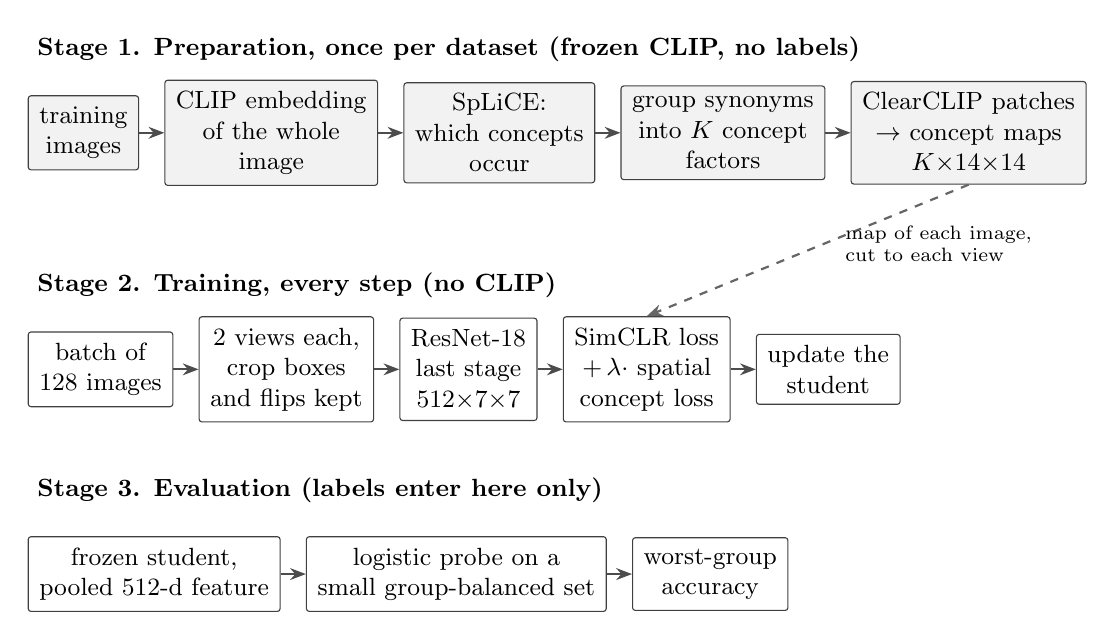
\begin{tikzpicture}[node distance=4mm and 3.2mm]
\node[font=\small\bfseries,anchor=west] (h1) at (0,0) {Stage 1. Preparation, once per dataset (frozen CLIP, no labels)};
\node[tbox,below=3mm of h1.south west,anchor=north west] (p1) {training\\images};
\node[tbox,right=of p1] (p2) {CLIP embedding\\of the whole\\image};
\node[tbox,right=of p2] (p3) {SpLiCE:\\which concepts\\occur};
\node[tbox,right=of p3] (p4) {group synonyms\\into $K$ concept\\factors};
\node[tbox,right=of p4] (p5) {ClearCLIP patches\\$\to$ concept maps\\$K{\times}14{\times}14$};
\draw[arr] (p1)--(p2); \draw[arr] (p2)--(p3); \draw[arr] (p3)--(p4); \draw[arr] (p4)--(p5);
\node[font=\small\bfseries,anchor=west] (h2) at (0,-3.0) {Stage 2. Training, every step (no CLIP)};
\node[box,below=3mm of h2.south west,anchor=north west] (t1) {batch of\\128 images};
\node[box,right=of t1] (t2) {2 views each,\\crop boxes\\and flips kept};
\node[box,right=of t2] (t3) {ResNet-18\\last stage\\$512{\times}7{\times}7$};
\node[box,right=of t3] (t4) {SimCLR loss\\$+\,\lambda\cdot$ spatial\\concept loss};
\node[box,right=of t4] (t5) {update the\\student};
\draw[arr] (t1)--(t2); \draw[arr] (t2)--(t3); \draw[arr] (t3)--(t4); \draw[arr] (t4)--(t5);
\draw[darr] (p5.south) -- (t4.north);
\node[font=\scriptsize,align=left,anchor=west] at ($(p5.south)!0.45!(t4.north)+(1.5mm,0)$) {map of each image,\\cut to each view};
\node[font=\small\bfseries,anchor=west] (h3) at (0,-5.6) {Stage 3. Evaluation (labels enter here only)};
\node[box,below=3mm of h3.south west,anchor=north west] (e1) {frozen student,\\pooled 512-d feature};
\node[box,right=of e1] (e2) {logistic probe on a\\small group-balanced set};
\node[box,right=of e2] (e3) {worst-group\\accuracy};
\draw[arr] (e1)--(e2); \draw[arr] (e2)--(e3);
\end{tikzpicture}
\caption{The three stages of SCD. After Stage~1 only the concept maps are kept; after Stage~2 only the ResNet-18 is kept. The maps, the projection head and every ridge fit are discarded. Concept discovery, map construction and SSL use no target or group annotations and no concept type.}
\label{fig:architecture}
\end{figure}

\subsection{Stage 1a: a concept vocabulary from SpLiCE}
SpLiCE gives a vocabulary of the concepts that occur in the training set, without annotating which of them are spurious. Given an image $x_i$ resized to 224 pixels, frozen CLIP produces the embedding $z_i\in\mathbb{R}^{512}$ of the \emph{whole} image. With the fixed SpLiCE mean $\mu$ and a row-normalized text dictionary $D\in\mathbb{R}^{V\times 512}$ of $V$ words, positive sparse regression gives
\begin{equation}
 u_i=\operatorname{norm}(z_i-\mu),\qquad
 c_i\in\arg\min_{c\geq0}\|u_i-D^\top c\|_2^2+\lambda_1\|c\|_1,
\end{equation}
with $\operatorname{norm}(v)=v/\lVert v\rVert_2$ and $\lambda_1=0.25$. About nine coordinates of $c_i$ are non-zero; a MetaShift image might give $c_i=0.41\,e_{\text{cat}}+0.30\,e_{\text{couch}}+0.12\,e_{\text{blanket}}+\ldots$, where $e_k$ is the coordinate of word $k$. SpLiCE runs on whole-image embeddings only. Its role is to decide \emph{which} words describe this dataset and how often; the locations come later from patch embeddings.

\subsection{Stage 1b: concept factors}
Words of the dictionary often name one visual content several times (\emph{cat}, \emph{kitten}, \emph{kitty}). If each word kept its own channel, synonyms would compete for the same pixels in the maps of Stage~1c and split the mass of one object over several names. We therefore group words into \emph{concept factors}. The L1 penalty of SpLiCE activates one of two synonyms per image, so synonyms rarely co-activate and their centred dictionary directions can lie far apart. Raw CLIP text embeddings $t^{\text{text}}_k$ keep synonyms close (cosine 0.85 to 0.94) and separate an object from its usual context (0.64 to 0.72). We keep words active on 0.2\% to 95\% of the training images and define the similarity of two words as
\begin{equation}
 s_{k\ell}=
 \begin{cases}
 \cos(t^{\text{text}}_k,t^{\text{text}}_\ell) & \text{if } \rho_{k\ell}\geq0.5,\\
 -1 & \text{otherwise,}
 \end{cases}
\end{equation}
where $\rho_{k\ell}$ is the correlation across training images of the responses $u_i^\top d_k$ and $u_i^\top d_\ell$. Average-linkage clustering on $1-s_{k\ell}$, cut at similarity 0.85, forms the groups. Average linkage joins two clusters only when their members agree on average, which stops the chains that a union of pairwise matches forms through a bird and its background.

A concept factor $F$ is one group, for example \{kitty, kitten, cat\}, \{canine, dog\} or \{couch, sofa\}. Its text direction is the normalized mean of its members' text embeddings,
\begin{equation}
 d_F=\operatorname{norm}\Big(\tfrac{1}{|F|}\textstyle\sum_{k\in F}\operatorname{norm}(t^{\text{text}}_k)\Big),
\end{equation}
and we keep factors active on 2\% to 90\% of the training images. Waterbirds has $K=242$ factors, MetaShift 130 and Spur-CIFAR10 147. The factors include the object classes and their contexts alike; nothing marks one of them as the class.

\subsection{Stage 1c: dense concept maps}
\label{sec:maps}
Stage~1c computes, for every training image, where each factor sits. This needs three decisions: which patch embeddings to read, at which resolution and how to turn patch scores into a map.

\paragraph{Patch embeddings that match text.}
CLIP's vision transformer cuts the image into patches and keeps one token per patch. Training aligns only the class token with text. In the last block the query--key attention of every patch concentrates on the same few global tokens \citep{zhou2022maskclip,wang2024sclip,darcet2024registers} and the residual branch adds this global signal to every patch, so a patch on the couch repeats the summary ``cat, couch, room'' of the whole image. ClearCLIP \citep{lan2024clearclip} changes only the last block. It drops the residual and feed-forward branches and replaces query--key attention by query--query attention, so a patch attends to patches that resemble it. With $X$ the normalized tokens entering this block, the patch embeddings in the text space are
\begin{equation}
 P=\operatorname{norm}\!\Big(\operatorname{LN}\big(\operatorname{softmax}(QQ^\top/\sqrt{d_h})\,V\,W_O\big)\,W_{\mathrm{proj}}\Big),
 \qquad Q=XW_Q,\; V=XW_V,
\end{equation}
applied per attention head and normalized per patch. Each patch $u$ gets a unit vector $p(u)\in\mathbb{R}^{512}$ in the space of the factor directions $d_F$. ClearCLIP needs no training and no labels.

\paragraph{Resolution: why the image is read at 448 pixels.}
The teacher is OpenCLIP ViT-B/32 \citep{radford2021clip}. Two properties of this model fix the resolution. First, its input is $224\times224$ pixels: it was trained at this size and its positional embeddings cover a $7\times7$ grid of patches. Second, a patch is 32 pixels wide, so a 224-pixel input gives $224/32=7$ patches per side. One CLIP patch then covers $\tfrac17$ of the image side and CLIP cannot resolve anything smaller than its patch: the head of a cat and the cushion next to it share one vector.

The training images of MetaShift and Waterbirds have arbitrary sizes, so every image has to be resized to some fixed size in any case. Table~\ref{tab:resolution} lists the options. Feeding the image at 224 pixels gives a $7\times7$ map. Feeding 448 pixels in one pass gives $14\times14$ patches, but CLIP then runs at a size it was not trained on and its positional embeddings must be interpolated. SCD resizes every image to $448\times448$ pixels and reads it through nine windows of $224\times224$ pixels at offsets $\{0,112,224\}$ in each direction (Figure~\ref{fig:windows}). Every window is a native 224-pixel CLIP input and yields $7\times7$ patches of 32 pixels, while 32 pixels are now $\tfrac{1}{14}$ of the image side. The map resolution doubles without any input that CLIP has not seen in training. The same sliding-window reading is the evaluation protocol of SCLIP and ClearCLIP for open-vocabulary segmentation \citep{wang2024sclip,lan2024clearclip}.

\begin{table}[htbp]
\centering\small
\caption{How the size of the image fed to CLIP ViT-B/32 determines the concept map. The patch is always 32 pixels.}
\label{tab:resolution}
\begin{tabularx}{\linewidth}{lllX}
\toprule
Input to CLIP & Patches & One patch covers & Consequence \\
\midrule
original image & -- & -- & arbitrary sizes; CLIP needs a fixed input \\
$224\times224$, one pass & $7\times7$ & $\tfrac17$ of the side & a small crop covers about $3\times3$ patches \\
$448\times448$, one pass & $14\times14$ & $\tfrac1{14}$ of the side & positional embeddings interpolated beyond training \\
$448\times448$, nine 224-px windows & $9\times(7\times7)$ & $\tfrac1{14}$ of the side & native input in every window; used by SCD \\
\bottomrule
\end{tabularx}
\end{table}

\begin{figure}[htbp]
\centering
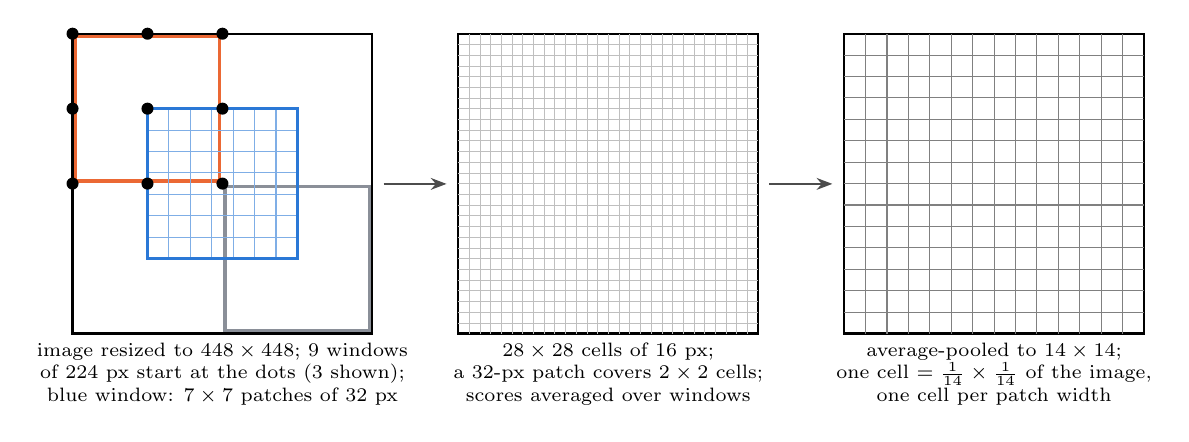
\begin{tikzpicture}
\begin{scope}[scale=0.0085]
\draw[thick] (0,0) rectangle (448,448);
\draw[very thick,couchc] (4,228) rectangle (220,444);
\draw[very thick,windowc] (228,4) rectangle (444,220);
\foreach \i in {1,...,6} {
  \draw[catc!60,thin] (112+\i*32,112) -- ++(0,224);
  \draw[catc!60,thin] (112,112+\i*32) -- ++(224,0);
}
\draw[very thick,catc] (112,112) rectangle ++(224,224);
\foreach \x in {0,112,224} { \foreach \y in {224,336,448} { \fill[black] (\x,\y) circle (9); } }
\node[font=\scriptsize,align=center,below] at (224,0) {image resized to $448\times448$; 9 windows\\of 224 px start at the dots (3 shown);\\blue window: $7\times7$ patches of 32 px};
\end{scope}
\begin{scope}[xshift=4.9cm,scale=0.0085]
\draw[thick] (0,0) rectangle (448,448);
\foreach \i in {1,...,27} { \draw[black!25,very thin] (\i*16,0) -- ++(0,448); \draw[black!25,very thin] (0,\i*16) -- ++(448,0); }
\node[font=\scriptsize,align=center,below] at (224,0) {$28\times28$ cells of 16 px;\\a 32-px patch covers $2\times2$ cells;\\scores averaged over windows};
\end{scope}
\begin{scope}[xshift=9.8cm,scale=0.0085]
\draw[thick] (0,0) rectangle (448,448);
\foreach \i in {1,...,13} { \draw[black!50,thin] (\i*32,0) -- ++(0,448); \draw[black!50,thin] (0,\i*32) -- ++(448,0); }
\node[font=\scriptsize,align=center,below] at (224,0) {average-pooled to $14\times14$;\\one cell $=\tfrac1{14}\times\tfrac1{14}$ of the image,\\one cell per patch width};
\end{scope}
\draw[arr] (3.95,1.9) -- (4.75,1.9);
\draw[arr] (8.85,1.9) -- (9.65,1.9);
\end{tikzpicture}
\caption{From windows to the $14\times14$ map. Left: the nine windows have their top-left corners at pixels 0, 112 and 224 in each direction (dots); three of them are drawn, the top-left (orange), the centre (blue, with its $7\times7$ patches) and the bottom-right (grey). Neighbouring windows overlap by half, so their patches fall on a 16-pixel grid (middle) and a cell is covered by one, two or four windows. Right: the averaged scores pooled to the $14\times14$ map.}
\label{fig:windows}
\end{figure}

\paragraph{Where $14\times14$ comes from.}
For every window and every patch $u$ we compute the cosine with every factor direction, $s_F(u)=p(u)^\top d_F$. Windows overlap by half their width, so the patches of neighbouring windows are shifted by 112 pixels, which is three and a half patches. Their borders therefore fall on a grid of 16-pixel cells, $448/16=28$ cells per side. Each patch spreads its scores onto its $2\times2$ cells, scores are averaged where windows overlap and the $28\times28$ grid is average-pooled to $14\times14$, one cell per patch width. The averaging over one, two or four windows also reduces the noise of single patches.

\paragraph{Why the map stops at $14\times14$.}
The resolution of the map is set by the student, which sees views of 20\% to 100\% of the image area (Section~\ref{sec:views}) and has a $7\times7$ feature map. A view that covers the whole image spans $14\times14$ cells, so each of its $7\times7$ targets averages $2\times2$ cells. The smallest view spans $\sqrt{0.2}\approx0.45$ of the image side, which is $0.45\times14\approx6$ cells per side: close to one map cell per student location, so even the smallest crop receives real, separately computed content. A $7\times7$ map would give the smallest crop about $3\times3$ cells, stretched over $7\times7$ locations and neighbouring student locations would receive identical blurred targets exactly on the views where an object fills half the view. A $28\times28$ map adds no resolution of its own, since its 16-pixel cells come from averaging 32-pixel patches and it takes four times the memory: the $14\times14$ maps take 87 MB for MetaShift and 455 MB for Waterbirds, against about 1.8 GB for Waterbirds at $28\times28$. Training holds the maps in memory.

\paragraph{The square resize keeps maps and views aligned.}
Resizing to $448\times448$ changes the aspect ratio of the image. The map covers the whole image and the crop box of a view is stored as fractions of the image side (Section~\ref{sec:views}). A fraction such as ``from 30\% to 70\% of the width'' is the same before and after any resize, so the box lands on the right cells of the map whatever the original size and shape of the image.

\paragraph{From scores to a map.}
At every cell $u$ of image $i$ the map distributes one unit of mass over the factors,
\begin{equation}
 M_{iF}(u)=\frac{\exp\!\big(s_{iF}(u)/\tau_M\big)}{\sum_{G=1}^{K}\exp\!\big(s_{iG}(u)/\tau_M\big)},\qquad \tau_M=0.01.
\end{equation}
The temperature is CLIP's own scale: CLIP multiplies its cosines by a learned logit scale of 100 before its zero-shot softmax \citep{radford2021clip}. Cosines of one patch with different words differ by a few hundredths and this scale lets one word win a cell. For illustration, a cell with cosines 0.27 with \emph{cat}, 0.25 with \emph{blanket} and 0.21 with \emph{couch} becomes about 88\% cat, 12\% blanket and 0.2\% couch; at $\tau_M=1$ the three would receive 34\%, 33\% and 32\%. When training loads the maps, every factor is standardized over all images and cells, $\tilde M_{iF}=(M_{iF}-m_F)/s_F$, so that frequent factors such as blanket or lawn do not dominate the squared error of Section~\ref{sec:loss}. The maps are stored once in float16 and take 40 seconds to compute for MetaShift on one GPU. Figure~\ref{fig:examples} shows maps of four MetaShift images.

\begin{figure}[htbp]
\centering
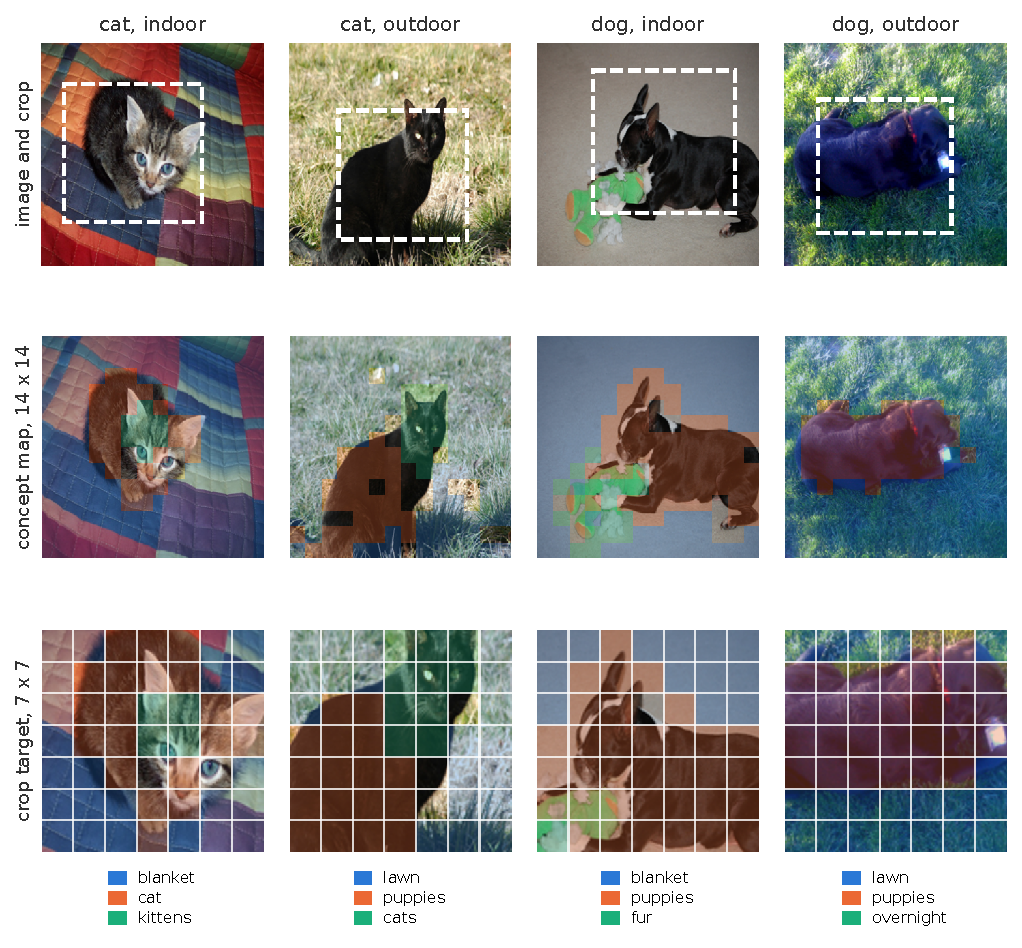
\includegraphics[width=\linewidth]{figures/spatial_map_examples.pdf}
\caption{Concept maps of MetaShift training images, one per group. Top: the image and one SimCLR crop (dashed). Middle: the factor that wins each cell of the $14\times14$ map, coloured for the image's three most frequent factors. Bottom: the crop's targets after warping to the student's $7\times7$ feature map (Section~\ref{sec:warp}). The teacher makes mistakes: part of the black cat in the second image is labelled ``puppies''. Class and group labels play no part in map construction or training.}
\label{fig:examples}
\end{figure}

\subsection{Stage 2a: views, crop boxes and the student feature map}
\label{sec:views}
Training is ordinary SimCLR on a ResNet-18 from random weights. Every image of a batch of 128 gives two views. The transform of a view applies a random crop of 20\% to 100\% of the image area with aspect ratio between 3:4 and 4:3, resized to $224\times224$; a horizontal flip with probability 0.5; colour jitter with probability 0.8 and greyscale with probability 0.2. Crop and flip are the only operations that move pixels, so the transform records for every view its crop box as fractions of the image (top $a$, left $b$, height $\eta$, width $\omega$) and its flip flag. These records tell which part of the concept map each view shows.

The ResNet-18 \citep{he2016resnet} halves the resolution five times and maps a view to $H\in\mathbb{R}^{512\times7\times7}$ at the output of its last residual stage, since $224/2^5=7$. Global average pooling gives the 512-dimensional feature $h$ that the probe reads after training and an MLP head maps $h$ to the 128-dimensional input of the SimCLR loss. The concept loss reads $H$ before pooling. Location $(r,c)$ of $H$ lies over the 32-pixel square $(r,c)$ of the view, so each of the 49 vectors can be asked about its own part of the view; class activation maps rest on the same property of the last feature map \citep{zhou2016cam}. After pooling, a cat and a couch in the same view become one vector; before pooling they still occupy different locations. This is why the concept loss reads the feature map and leaves the pooled feature to SimCLR. The probe reads the pooled feature of the same backbone that the loss shapes.

The student's $7\times7$ grid and the $7\times7$ patch grid of a CLIP window have the same size for different reasons ($224/2^5$ and $224/32$). The two grids never meet: CLIP's grids are assembled into the $14\times14$ map of the whole image and the warping below resamples that map to the student's grid of each view.

\subsection{Stage 2b: warping the map to each view}
\label{sec:warp}
For a view with box $(a,b,\eta,\omega)$, the box in map coordinates is $[14b,\,14(b+\omega)]\times[14a,\,14(a+\eta)]$. RoIAlign \citep{he2017maskrcnn} divides it into $7\times7$ bins and averages $2\times2$ bilinear samples of $\tilde M_i$ inside each bin; a flipped view gets its targets mirrored along the width. The result is the target tensor of view $v$,
\begin{equation}
 T^{(v)}=\operatorname{flip}^{\,\phi_v}\!\Big(\operatorname{RoIAlign}\big(\tilde M_i,\ \text{box}_v,\ 7\times7\big)\Big)\in\mathbb{R}^{K\times7\times7},
\end{equation}
with $\phi_v\in\{0,1\}$ the flip flag. Cell $(r,c)$ of $T^{(v)}$ describes exactly the part of the view that student location $(r,c)$ looks at (Figure~\ref{fig:warp}). RoIAlign reads the map at fractional positions, so a crop that starts inside a cell receives the correct values.

\begin{figure}[htbp]
\centering
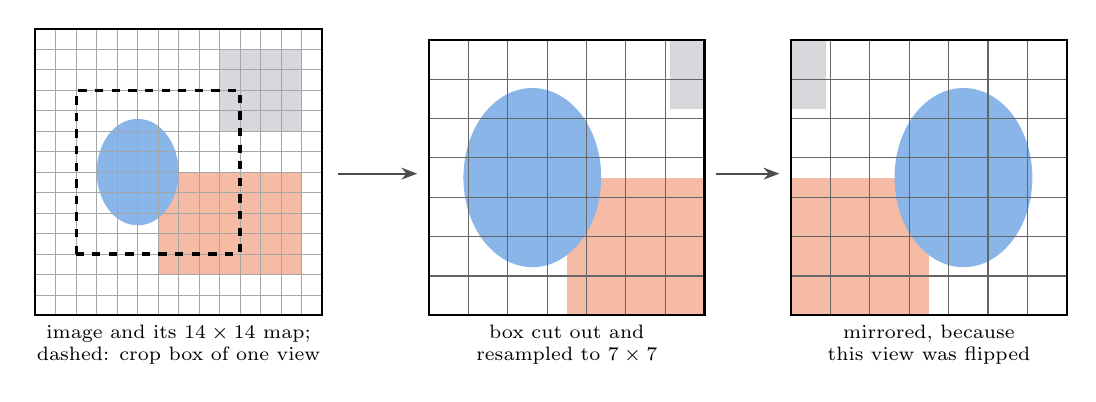
\begin{tikzpicture}
\begin{scope}[x=0.26cm,y=0.26cm]
\toyscene
\draw[black!35,very thin] (0,0) grid[step=1] (14,14);
\draw[thick] (0,0) rectangle (14,14);
\draw[very thick,dashed] (2,3) rectangle (10,11);
\node[font=\scriptsize,align=center,below] at (7,0) {image and its $14\times14$ map;\\dashed: crop box of one view};
\end{scope}
\begin{scope}[xshift=5.0cm]
\begin{scope}[x=0.4375cm,y=0.4375cm,shift={(-2,-3)}]
\clip (2,3) rectangle (10,11);
\toyscene
\end{scope}
\draw[black!60,thin] (0,0) grid[step=0.5cm] (3.5,3.5);
\draw[thick] (0,0) rectangle (3.5,3.5);
\node[font=\scriptsize,align=center,below] at (1.75,0) {box cut out and\\resampled to $7\times7$};
\end{scope}
\begin{scope}[xshift=9.6cm]
\begin{scope}[x=-0.4375cm,y=0.4375cm,shift={(-10,-3)}]
\clip (2,3) rectangle (10,11);
\toyscene
\end{scope}
\draw[black!60,thin] (0,0) grid[step=0.5cm] (3.5,3.5);
\draw[thick] (0,0) rectangle (3.5,3.5);
\node[font=\scriptsize,align=center,below] at (1.75,0) {mirrored, because\\this view was flipped};
\end{scope}
\draw[arr] (3.85,1.8) -- (4.85,1.8);
\draw[arr] (8.65,1.8) -- (9.45,1.8);
\end{tikzpicture}
\caption{Warping the map to one view (toy scene). All $K$ channels of the map are cut and resampled in the same way; the figure colours each cell by its winning factor: \textcolor{catc}{$\blacksquare$}~cat, \textcolor{couchc}{$\blacksquare$}~couch and \textcolor{windowc}{$\blacksquare$}~window.}
\label{fig:warp}
\end{figure}

\subsection{Stage 2c: the cross-fitted spatial concept loss}
\label{sec:loss}
\paragraph{Question--answer pairs.}
Every location $u$ of every view $v$ forms one pair: a unit-norm feature row $r=\operatorname{norm}(H^{(v)}(u))\in\mathbb{R}^{512}$, what the student sees there and a target $t=T^{(v)}(u)\in\mathbb{R}^{K}$, which concepts the teacher's map places there. The 128 images of a batch are split into halves $A$ and $B$ of 64 images, with both views of an image in the same half. Each half holds $64\times2\times49=6{,}272$ pairs. Stacking them gives $R_A\in\mathbb{R}^{6272\times512}$ and $T_A\in\mathbb{R}^{6272\times K}$; Table~\ref{tab:rows} shows a few rows for MetaShift.

\begin{table}[htbp]
\centering\small
\caption{Rows of half $A$ (MetaShift, $K=130$). Feature values and targets are illustrative; targets are standardized, so 0 is the average presence of a factor and positive values mark cells where it is more present than average.}
\label{tab:rows}
\footnotesize\setlength{\tabcolsep}{4pt}
\begin{tabular}{lll}
\toprule
Source of the row & $r\in\mathbb{R}^{512}$ (student) & $t\in\mathbb{R}^{130}$ (map): cat, couch, lawn, \ldots \\
\midrule
cat on couch, view 1, location (3,2) & $(0.04,-0.11,\ldots)$ & $(\phantom{-}2.1,-0.3,-0.4,\ldots)$ \\
cat on couch, view 1, location (5,5) & $(0.02,\phantom{-}0.07,\ldots)$ & $(-0.5,\phantom{-}2.4,-0.4,\ldots)$ \\
cat on couch, view 2, location (3,4) & $(0.05,-0.09,\ldots)$ & $(\phantom{-}1.8,-0.1,-0.4,\ldots)$ \\
dog on lawn, view 1, location (6,1) & $(-0.03,\phantom{-}0.01,\ldots)$ & $(-0.5,-0.3,\phantom{-}2.7,\ldots)$ \\
\multicolumn{3}{c}{\ldots\ 6{,}272 rows in total} \\
\bottomrule
\end{tabular}
\end{table}

\paragraph{Why a readout is needed.}
The 512 coordinates of the student do not correspond to the $K$ factors and the student should be free to arrange its feature space. A linear map $W\in\mathbb{R}^{512\times K}$ translates features into concept values: the predicted value of \emph{cat} at a location is the projection of its feature row on the cat column of $W$. A linear readout matches the evaluation, where a linear probe reads the features, so concepts have to become \emph{linearly} readable.

\paragraph{Why the readout is refitted and cross-fitted.}
A readout trained by gradient descent alongside the student could store a target per image: a deep network can fit arbitrary targets on a small dataset \citep{zhang2017rethinking} and MetaShift has 1,700 training images. A student that recognizes ``this is image 371'' and stores its answers lowers such a loss without learning any concept. SCD therefore fits the readout in closed form on half $A$ and scores it on half $B$, whose images the fit has never seen. With $\Omega_A$ the diagonal matrix of per-row loss weights, $\bar r_A$ and $\bar t_A$ the weighted means of rows and targets in $A$ and $\bar R_A=R_A-\mathbf{1}\bar r_A^\top$, the weighted ridge regression is
\begin{equation}
 W_A=\big(\bar R_A^\top\Omega_A\bar R_A+\rho I\big)^{-1}\bar R_A^\top\Omega_A\big(T_A-\mathbf{1}\bar t_A^\top\big)\in\mathbb{R}^{512\times K},
 \qquad \rho=1,
\end{equation}
one $512\times512$ linear system \citep{hoerl1970ridge}. The fit predicts every location of $B$,
\begin{equation}
 \hat T_B=(R_B-\mathbf{1}\bar r_A^\top)\,W_A+\mathbf{1}\bar t_A^\top,
\end{equation}
and the reverse fit $W_B$ predicts $A$ (Figure~\ref{fig:crossfit}). The loss is the held-out squared error, averaged over the two directions,
\begin{equation}
 \mathcal{L}_{\mathrm{spatial}}=\frac{1}{2}\sum_{(S,S')\in\{(A,B),(B,A)\}}
 \frac{\sum_{v\in S'}\omega_v\,\frac{1}{49K}\big\lVert\hat T^{(v)}-T^{(v)}\big\rVert_2^2}{\sum_{v\in S'}\omega_v},
\end{equation}
where $\hat T^{(v)}$ collects the predictions of the 49 locations of view $v$ by the fit on the other half and $\omega_v$ is its loss weight. Gradients flow through the prediction and through the solve for $W_A$ into $H$ and the ResNet weights \citep{bertinetto2019r2d2}. The readout has no parameters of its own; it is solved again in every step from the current features and discarded afterwards.

\begin{figure}[htbp]
\centering
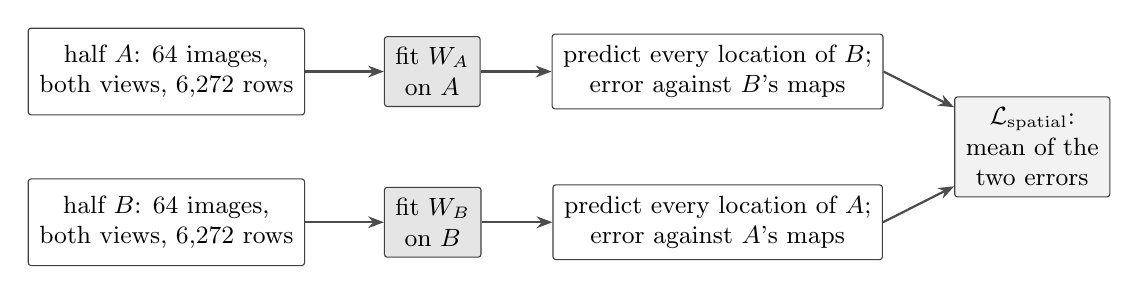
\begin{tikzpicture}[node distance=4mm]
\node[box,minimum width=26mm,minimum height=11mm] (A) {half $A$: 64 images,\\both views, 6,272 rows};
\node[box,minimum width=26mm,minimum height=11mm,below=8mm of A] (B) {half $B$: 64 images,\\both views, 6,272 rows};
\node[lbox,right=10mm of A] (fitA) {fit $W_A$\\on $A$};
\node[lbox,right=10mm of B] (fitB) {fit $W_B$\\on $B$};
\node[box,right=9mm of fitA] (predB) {predict every location of $B$;\\error against $B$'s maps};
\node[box,right=9mm of fitB] (predA) {predict every location of $A$;\\error against $A$'s maps};
\node[tbox,right=9mm of $(predB.east)!0.5!(predA.east)$] (loss) {$\mathcal L_{\text{spatial}}$:\\mean of the\\two errors};
\draw[arr] (A)--(fitA); \draw[arr] (B)--(fitB);
\draw[arr] (fitA)--(predB); \draw[arr] (fitB)--(predA);
\draw[arr] (predB.east)--(loss); \draw[arr] (predA.east)--(loss);
\end{tikzpicture}
\caption{Cross-fitting. Each readout is scored only on images it was not fitted on. Gradients pass through the solve and the prediction into the backbone.}
\label{fig:crossfit}
\end{figure}

\paragraph{Two ways to lower the loss.}
Consider two students. The first memorizes: it gives every image $i$ its own feature direction $e_i$, orthogonal to the directions of other images and $W_A$ maps each $e_i$ of half $A$ to that image's targets. On a location of an image $j$ in half $B$, $e_j$ is orthogonal to every direction that $W_A$ was fitted on, so the prediction collapses to about $\bar t_A$, the average target of $A$. Since the targets are standardized, this prediction has an error close to 1, the error of predicting the mean. Memorization earns nothing. The second student uses shared codes: a cat direction that appears on cat locations of every image and a couch direction on couch locations. $W_A$ learns ``cat direction $\mapsto$ cat value'' from the cats of $A$ and the same rule holds for the cats of $B$. Only this second kind of feature lowers $\mathcal{L}_{\mathrm{spatial}}$. Because the targets have unit variance, $1-\mathcal{L}_{\mathrm{spatial}}$ is the held-out explained variance, which we log during training.

\paragraph{Design choices of the loss.}
\begin{itemize}
\item \textbf{Unit-norm rows with an absolute ridge.} A student that could shrink its features would weaken the ridge penalty and let the readout overfit. Unit rows fix the scale and $\rho=1$ keeps the $512\times512$ system well conditioned.
\item \textbf{Both views of an image in one half.} Otherwise half $B$ would contain the second view of an image of half $A$ and recognizing the image would pay off again.
\item \textbf{Locations as rows.} Each half has $6{,}272$ rows for 512 unknowns per factor, a well-posed fit at batch size 128. A readout on pooled features would have 128 rows per half.
\item \textbf{Precision.} The network runs under float16 autocast; the solve and the loss run in float32.
\end{itemize}

\paragraph{Hold-out images.}
A fixed fifth of the training images (340 on MetaShift) carries loss weight $\omega_v=0$: their rows shape no readout and enter no error, while SimCLR trains on them as usual. After training they measure whether the student carries concepts to images outside the concept loss (Section~\ref{sec:capture}).

\subsection{The complete objective}
The SimCLR term is unchanged. With $g_v$ the normalized projection of view $v$, $v^+$ the other view of the same image and $\tau=0.05$, the NT-Xent loss \citep{oord2018cpc,chen2020simclr} over the $2B=256$ views of a batch is
\begin{equation}
 \mathcal{L}_{\mathrm{SimCLR}}=-\frac{1}{2B}\sum_{v=1}^{2B}\log\frac{\exp(g_v^\top g_{v^+}/\tau)}{\sum_{w\neq v}\exp(g_v^\top g_w/\tau)}.
\end{equation}
Each view has one positive (the other view of its image) and 254 negatives, among them views of other cats. SimCLR rewards every feature that separates images and has no reason to separate a cat from the couch it usually sits on; the spatial loss adds that reason. The training objective is
\begin{equation}
 \mathcal{L}=\mathcal{L}_{\mathrm{SimCLR}}+\lambda(e)\,\mathcal{L}_{\mathrm{spatial}},\qquad
 \lambda(e)=\begin{cases}0,& e\le10,\\ 5\,(e-10)/10,& 10<e<20,\\ 5,& e\ge20,\end{cases}
\end{equation}
with $e$ the epoch. SimCLR first forms usable features, then the concept loss rises to its full weight.

\section{SCD and CoSpRo}
\label{sec:cospro}
Both methods use the same frozen CLIP/SpLiCE vocabulary, the same SimCLR student and the same evaluation. They differ in what the teacher computes and in how it reaches the student (Table~\ref{tab:compare}).

\paragraph{The teacher signal.} CoSpRo computes \emph{relations between images}. For a concept group $G$ it removes the span $Q_G$ from the centred CLIP embeddings, $u_i^{-G}=\operatorname{norm}(u_i-Q_GQ_G^\top u_i)$, keeps pairs whose similarity rises, filters them by activation contrast, residual concept agreement and synthetic nulls and stores a sparse graph with a distribution $p_T(j\mid i)$ over donor images (Figure~\ref{fig:edges}). SCD computes a \emph{description of each location of each image}: a concept map. CoSpRo's signal is one number per image pair; SCD's signal is $K$ numbers per cell, about $196K$ values per image.

\paragraph{The prior.} CoSpRo searches for relations that appear when a concept is removed. This helps when the spurious attribute is a removable context concept and the class survives the removal. The same projection can remove object information: on Waterbirds 46\% of the graph mass of waterbirds on land connects images of the other class. SCD removes nothing and ranks no concept above another. The cat and the couch enter the loss as two factors with the same weight.

\paragraph{How the student is shaped.} CoSpRo acts on the pooled features: graph-aware batches place teacher neighbours together and a relational KL loss asks the student's similarity distribution to reproduce $p_T$. Only anchors with a donor in the batch contribute. SCD acts on the feature map before pooling: every location of every view of every image contributes in every step.

\paragraph{Memorization.} CoSpRo's targets are relations between specific images, which the student could satisfy by memorizing those pairs. SCD's cross-fit scores every readout on images it has not seen, so only codes shared across images lower the loss; the hold-out images confirm that the concepts transfer (Section~\ref{sec:capture}).

\paragraph{Cost and scope.} CoSpRo's graph construction evaluates candidate pairs for every concept group and calibrates every group against null groups. SCD's maps take 40 seconds for MetaShift and add no tuned threshold beyond the factor grouping. CoSpRo improved Waterbirds; SCD improves Waterbirds, MetaShift and Spur-CIFAR10 (Section~\ref{sec:vscospro}).

\begin{table}[htbp]
\centering\small
\caption{CoSpRo and SCD side by side.}
\label{tab:compare}
\begin{tabularx}{\linewidth}{lXX}
\toprule
& CoSpRo & SCD \\
\midrule
Teacher output & sparse graph of image pairs with weights & dense map of $K$ concept factors per image \\
Teacher computation & subspace removal, filters, null calibration & ClearCLIP patch scores, 9 windows, softmax \\
Assumption about the spurious attribute & a removable concept; its removal reveals same-class pairs & none; all concepts enter alike \\
Student signal & relational KL on pooled features & cross-fitted regression on the $7\times7$ feature map \\
Batches & graph-aware sampler & ordinary random batches \\
Rows per step & anchors with a donor in the batch & $2\times6{,}272$ locations \\
Protection against memorization & none & readout scored on the other half of the batch \\
Effect on WGA & Waterbirds only & Waterbirds, MetaShift, Spur-CIFAR10 \\
\bottomrule
\end{tabularx}
\end{table}

\begin{figure}[htbp]
\centering
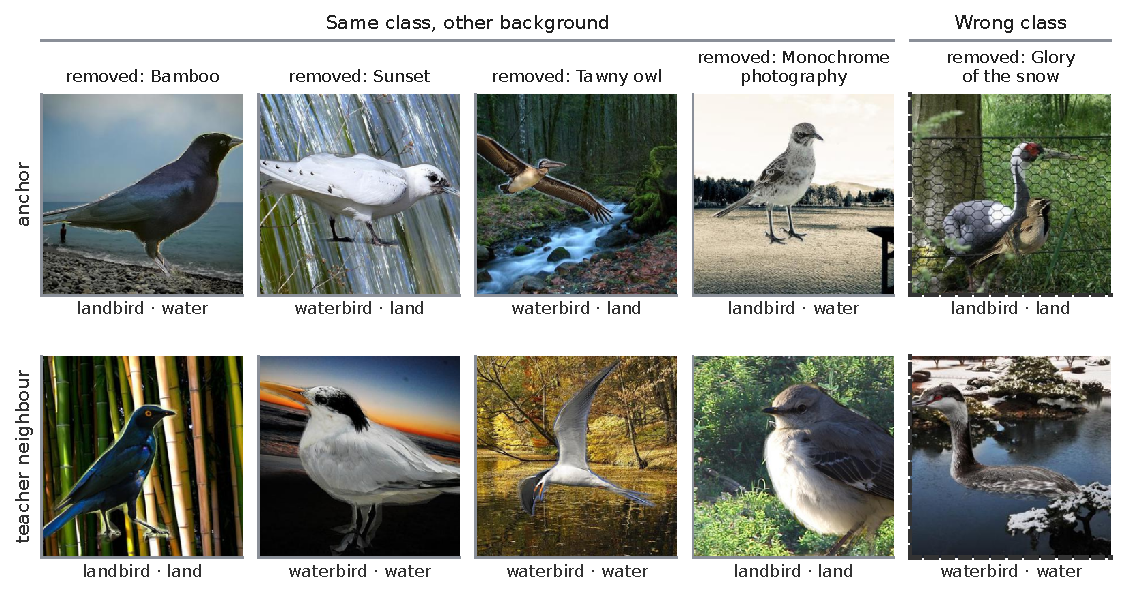
\includegraphics[width=\linewidth]{../../paper/figures/edge_examples.pdf}
\caption{CoSpRo's teacher signal for comparison with Figure~\ref{fig:examples}: retained graph edges on Waterbirds. Each column pairs an anchor (top) with its teacher neighbour (bottom) and names the concept whose removal produced the edge. The dashed pair on the right connects images of different classes. SCD replaces these pairwise relations by per-location concept maps.}
\label{fig:edges}
\end{figure}

\section{Experimental Protocol}
We evaluate on Waterbirds (4,795 training images; \citealp{sagawa2020groupdro}), MetaShift cats and dogs (1,700 training images; \citealp{liang2022metashift}) and Spur-CIFAR10, a CIFAR-10 variant \citep{krizhevsky2009cifar} in which a 2-pixel coloured line agrees with the class on 95\% of the 45,000 training images and on 10\% of the 5,000 validation images. Each dataset gets its own concept factors and maps from its training images. On Spur-CIFAR10 the 32-pixel images are upsampled to 448 pixels for the maps and the student's last feature map is $4\times4$.

We pretrain a randomly initialized ResNet-18 for 500 epochs with batch size 128, SGD with learning rate 0.01 decayed by 0.1 at epochs 350, 400 and 450, weight decay $10^{-4}$ and SimCLR temperature 0.05, with the same augmentations for every method. The protocol follows CoSpRo, LateTVG and LA-SSL, which pretrain on the dataset's own images, so that every method sees the same images and budget. The concept loss uses ridge $\rho=1$, maximum weight 5 and the 20\% hold-out. We report six student seeds on Waterbirds and MetaShift and two on Spur-CIFAR10.

Frozen student features are evaluated every 25 epochs with the same logistic probe (L2 coefficient 0.001), fitted on a group-balanced subset of the training split: 224 images on Waterbirds, 400 on MetaShift and 1,400 on Spur-CIFAR10. Group labels are used for this probe and its evaluation only. Unless stated otherwise each value is the mean of the last four probes (epochs 425 to 500), which damps single-probe noise on the small MetaShift validation groups (72 images each, so one image is 1.4 points of a group's accuracy). For the matched comparison with CoSpRo we also report the single probe at epoch 500, the protocol of the CoSpRo paper. We report mean and sample standard deviation across student seeds. All SCD results are validation results; held-out test runs with a locked probe are in progress.

\section{Results}
\subsection{SCD against SimCLR on three datasets}
\begin{table}[htbp]
\centering\small
\setlength{\tabcolsep}{3.5pt}
\caption{Validation evaluation, mean of the last four probes (SSL epochs 425--500). Waterbirds and MetaShift use seeds 1--6, Spur-CIFAR10 seeds 1--2. Shuffled maps give every image another image's maps. Values are percentages (mean $\pm$ sample standard deviation).}
\begin{tabular}{lrrrrrr}
\toprule
& \multicolumn{2}{c}{Waterbirds} & \multicolumn{2}{c}{MetaShift} & \multicolumn{2}{c}{Spur-CIFAR10} \\
Method & Avg. & WGA & Avg. & WGA & Avg. & WGA \\
\midrule
SimCLR & $52.44\pm1.07$ & $46.66\pm1.89$ & $55.16\pm3.99$ & $44.33\pm7.31$ & $59.55\pm0.23$ & $15.63\pm1.04$ \\
Shuffled maps & $52.79\pm2.71$ & $47.50\pm2.49$ & $56.08\pm2.23$ & $45.08\pm2.91$ & $55.90\pm0.71$ & $17.25\pm1.98$ \\
\textbf{SCD} & $\textbf{60.32}\pm\textbf{2.66}$ & $\textbf{52.76}\pm\textbf{4.68}$ & $\textbf{61.15}\pm\textbf{2.95}$ & $\textbf{51.10}\pm\textbf{5.44}$ & $\textbf{69.32}\pm\textbf{1.01}$ & $\textbf{38.13}\pm\textbf{0.51}$ \\
\bottomrule
\end{tabular}
\label{tab:main}
\end{table}

SCD achieves higher mean WGA than SimCLR by 6.10 points on Waterbirds, 6.77 on MetaShift and 22.50 on Spur-CIFAR10 (Table~\ref{tab:main}). The corresponding average-accuracy differences are $+7.88$, $+5.99$ and $+9.77$ points. SCD is ahead of SimCLR on five of six paired seeds on Waterbirds and MetaShift and on both Spur-CIFAR10 seeds (Figure~\ref{fig:paired}, which also shows CoSpRo). The shuffled-map control trains the same loss on maps of other images: it keeps the statistics of the targets and removes their link to the image content, in the manner of the control tasks of the probing literature \citep{hewitt2019control}. It stays within one point of SimCLR's WGA on Waterbirds and MetaShift and within 1.6 points on Spur-CIFAR10, so the gain comes from the content of each image's own maps. Seed variation is large on MetaShift, whose validation groups hold 72 images each. The weight $\lambda_{\max}=5$ and the hold-out were chosen on the validation splits of MetaShift and Waterbirds with seeds 1--4; seeds 5 and 6 ran afterwards with the settings fixed.

\begin{figure}[htbp]
\centering
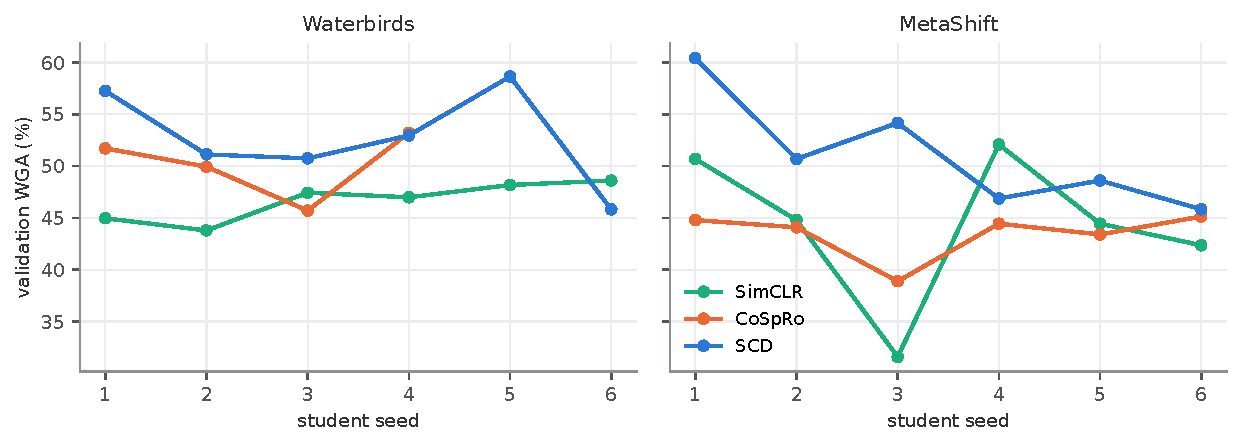
\includegraphics[width=\linewidth]{figures/scd_paired_seeds.pdf}
\caption{Validation WGA per student seed for SimCLR, CoSpRo and SCD, mean of the last four probes. CoSpRo has seeds 1--4 on Waterbirds; on MetaShift seeds 1--6 of its ten are shown.}
\label{fig:paired}
\end{figure}

\subsection{SCD against CoSpRo}
\label{sec:vscospro}
The SimCLR runs of seeds 1--4 on Waterbirds are shared by the CoSpRo study and this study, so the CoSpRo paper's validation protocol (single probe at epoch 500, seeds 1--4) gives a matched comparison (Table~\ref{tab:cospro}). SCD reaches $53.06$ WGA against $50.00$ for CoSpRo and $45.54$ for SimCLR; the average accuracy rises from 53.46 to 60.28. The paired WGA differences between SCD and CoSpRo are $+6.28$, $+1.13$, $+5.05$ and $-0.21$ points. The comparison favours SCD on average and on three of four seeds, with a margin of about one seed standard deviation.

\begin{table}[htbp]
\centering\small
\caption{Matched Waterbirds comparison: validation, single probe at SSL epoch 500, seeds 1--4, the protocol of the CoSpRo paper. Per-seed values are WGA; the SimCLR runs are shared by both studies.}
\label{tab:cospro}
\begin{tabular}{lrrrrrr}
\toprule
Method & Avg. & WGA & Seed 1 & Seed 2 & Seed 3 & Seed 4 \\
\midrule
SimCLR & $52.11$ & $45.54\pm1.71$ & 44.54 & 43.68 & 47.32 & 46.62 \\
CoSpRo + KL & $53.46$ & $50.00\pm3.23$ & 51.61 & 50.00 & 45.49 & 52.89 \\
\textbf{SCD} & $\textbf{60.28}$ & $\textbf{53.06}\pm\textbf{3.35}$ & 57.89 & 51.13 & 50.54 & 52.68 \\
\bottomrule
\end{tabular}
\end{table}

Across datasets the difference is larger (Table~\ref{tab:cospro_all}). CoSpRo stayed at the SimCLR level on MetaShift over ten seeds ($42.9$ against $44.4$) and reached $19.6$ WGA on one Spur-CIFAR10 seed, while SCD gains 6.8 and 22.5 points there. On the held-out Waterbirds test split CoSpRo reached $50.64\pm1.97$ against $46.82\pm3.65$ for SimCLR; the matched test runs of SCD are in progress, so the test comparison remains open.

\begin{table}[htbp]
\centering\small
\caption{Validation WGA of SimCLR, CoSpRo and SCD on the three datasets, mean of the last four probes. Seeds in brackets. The MetaShift CoSpRo study ran its own ten SimCLR seeds, which reach 44.41 WGA.}
\label{tab:cospro_all}
\begin{tabular}{lrrr}
\toprule
Method & Waterbirds & MetaShift & Spur-CIFAR10 \\
\midrule
SimCLR & $46.66\pm1.89$ (6) & $44.33\pm7.31$ (6) & $15.63\pm1.04$ (2) \\
CoSpRo + KL & $50.14\pm3.25$ (4) & $42.92\pm2.62$ (10) & $19.6$ (1) \\
\textbf{SCD} & $\textbf{52.76}\pm\textbf{4.68}$ (6) & $\textbf{51.10}\pm\textbf{5.44}$ (6) & $\textbf{38.13}\pm\textbf{0.51}$ (2) \\
\bottomrule
\end{tabular}
\end{table}

The differences of Section~\ref{sec:cospro} explain this pattern. CoSpRo's projection reveals same-class pairs when the removed concept is the background and the bird survives the removal, which holds best for Waterbirds. SCD needs no such condition: its targets describe every concept of every location and its cross-fit keeps the signal from turning into memorized pairs on the 1,700 MetaShift images.

\subsection{Do named concepts and their locations add value beyond CLIP?}
Two controls isolate the parts of SCD. The principal-component control replaces the concept maps by as many principal components of the dense ClearCLIP patch embeddings as there are factors, computed over the same cells and trained with the same loss. It keeps the dense CLIP information of the teacher and removes the concept names. The image-level control regresses each image's SpLiCE factor activations from the pooled features with the same cross-fitted ridge, weight and hold-out. It keeps the concepts and removes their locations.

\begin{table}[htbp]
\centering\small
\caption{Controls, validation at epochs 425--500, seeds 1--4. Mean $\pm$ sample standard deviation in percent. All share the backbone, optimization, hold-out and probing protocol. $^\dagger$Seeds 1--2. $^\ddagger$Factors from a 5\% frequency band (70 on Waterbirds, 24 on MetaShift).}
\begin{tabular}{lrrrr}
\toprule
& \multicolumn{2}{c}{Waterbirds} & \multicolumn{2}{c}{MetaShift} \\
Method & Avg. & WGA & Avg. & WGA \\
\midrule
SimCLR & $52.25\pm1.21$ & $45.80\pm1.71$ & $54.80\pm4.81$ & $44.79\pm9.35$ \\
Shuffled maps & $52.60\pm3.48$ & $46.73\pm2.70$ & $55.62\pm2.27$ & $45.31\pm3.38$ \\
CLIP principal-component maps & $58.07\pm0.94$ & $53.57\pm1.93$ & $56.29\pm2.23$ & $44.44\pm7.37$ \\
Image-level concept regression$^\ddagger$ & $57.96\pm3.95$ & $50.37\pm8.98$ & $61.68\pm0.18^\dagger$ & $47.22\pm3.93^\dagger$ \\
SCD & $60.15\pm2.46$ & $53.02\pm2.98$ & $62.22\pm2.97$ & $53.04\pm5.75$ \\
\bottomrule
\end{tabular}
\label{tab:controls}
\end{table}

On MetaShift, SCD has 8.59-point higher mean WGA than the principal-component maps and is ahead on all four seeds; the paired differences are $+15.97$, $+1.39$, $+4.17$ and $+12.85$ points (Table~\ref{tab:controls}). The principal-component maps stay at the SimCLR level there. On Waterbirds the two tie ($-0.54$ WGA, $+2.07$ Avg.): birds against land and water are among the strongest directions of CLIP's patch embeddings, so its leading components carry them, while cats against dogs and couches against lawns are weaker directions that only the named concepts single out. SCD exceeds the image-level regression by 2.66 WGA points on Waterbirds and 8.33 on the two MetaShift seeds; on Spur-CIFAR10 the image-level regression reaches $29.39$ WGA against $38.13$ (two seeds each). Image-level heads also store the targets of MetaShift's training images: at weight 10 the concept score on images inside the loss reaches 0.60 while the score on held-out images falls to 0.04. The spatial loss shows no such gap (Section~\ref{sec:capture}).

A concept ablation tests which concepts carry the MetaShift gain. It uses word lists we chose and lies outside the method. Over seeds 1--4, leaving out the 21 animal factors (cat, dog, breeds, pet, paws, fur) gives $46.61\pm5.75$ WGA and leaving out the 20 scene factors (couch, lawn, bed, window, desk, bench and others) $47.92\pm2.81$, against $53.04\pm5.75$ with all factors and $45.31\pm3.38$ with shuffled maps. Both ablations lose most of the gain and differ by less than the seed noise: the gain needs the object and the scene concepts together, which is what lets the student tell them apart.

\subsection{Training dynamics and groups}
The worst-group advantage of SCD holds across training (Figure~\ref{fig:curves}). On MetaShift its smoothed mean WGA leads SimCLR and CoSpRo at every probe, while CoSpRo falls below SimCLR from epoch 175 onward. On Waterbirds CoSpRo rises first and leads from epoch 50 to 125; the two alternate up to epoch 200 and from epoch 225 SCD stays ahead to the end of training. SCD leads both methods in average accuracy at every probe on both datasets, while CoSpRo stays within two points of SimCLR.

\begin{figure}[htbp]
\centering
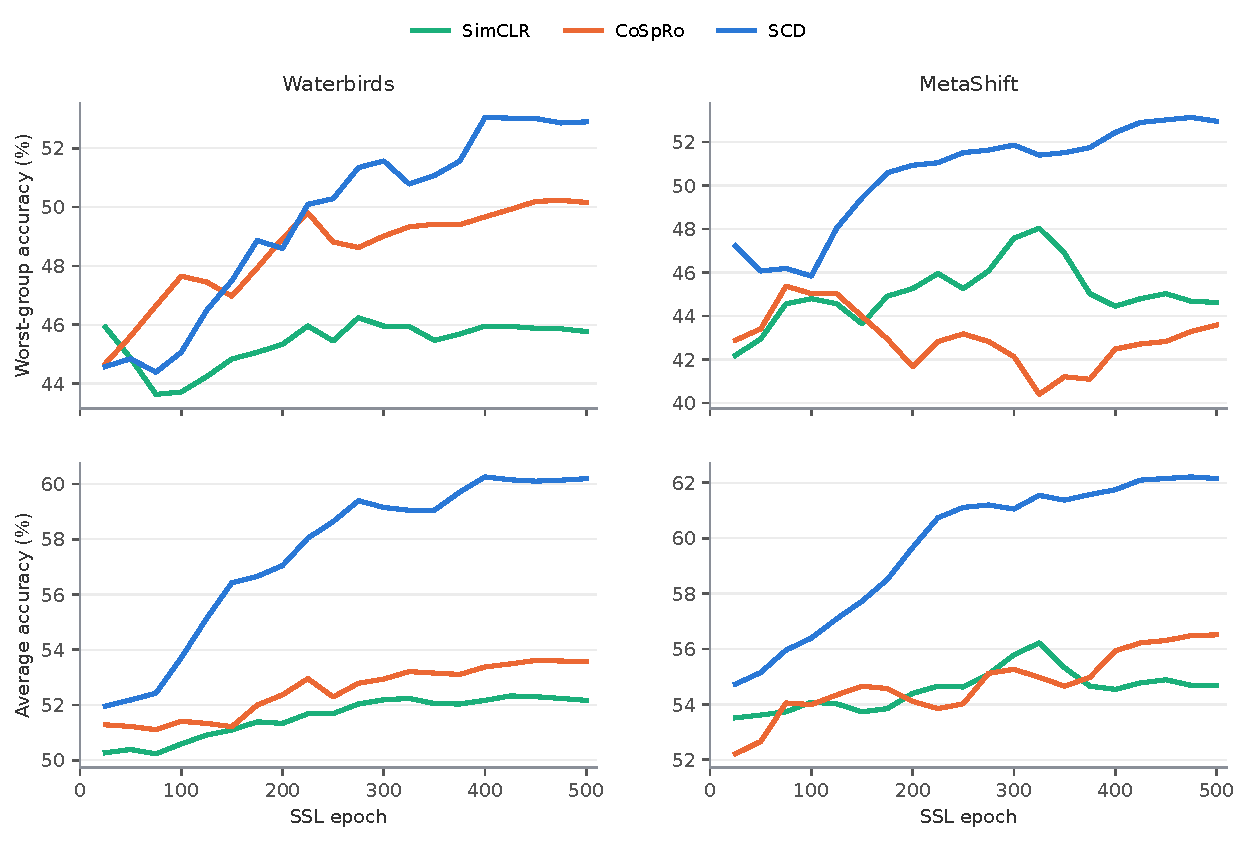
\includegraphics[width=\linewidth]{figures/scd_training_curves.pdf}
\caption{Validation accuracy during SSL training for SimCLR, CoSpRo and SCD. Each line is the mean over seeds 1--4 of the periodic linear probes, run every 25 epochs, smoothed with a three-point moving average. Top: worst-group accuracy. Bottom: average accuracy.}
\label{fig:curves}
\end{figure}

The gain extends to the minority groups (Figure~\ref{fig:groups}): on MetaShift cats outdoors rise from 47.0 to 51.2 and dogs indoors from 52.8 to 57.2; on Waterbirds landbirds on water rise from 53.6 to 65.1. SCD raises every group on both datasets. CoSpRo raises the land groups of Waterbirds (landbirds on land 47.6 to 51.0, waterbirds on land 53.8 to 56.6) and leaves landbirds on water at 52.3; on MetaShift its groups stay within the seed spread of SimCLR.

\begin{figure}[htbp]
\centering
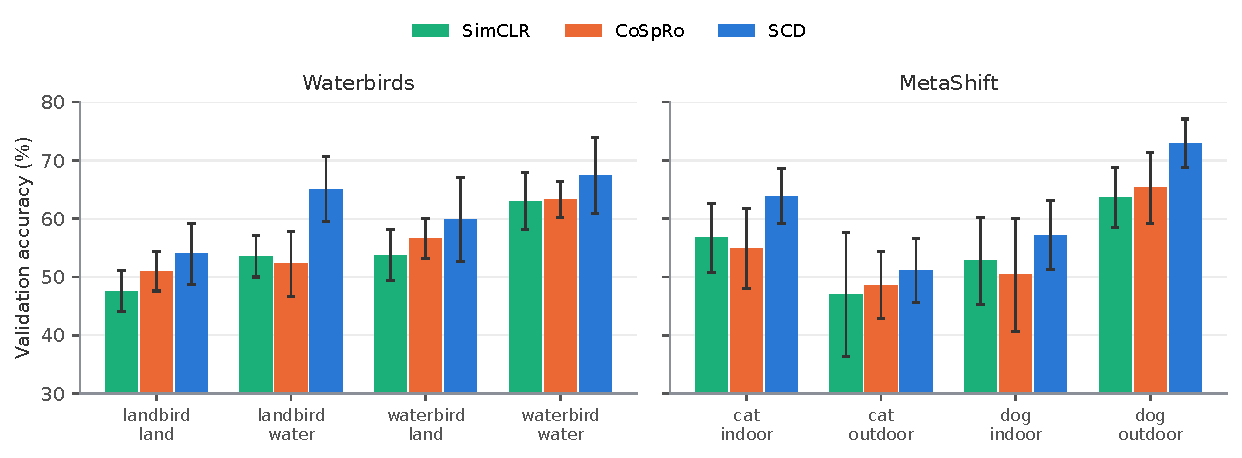
\includegraphics[width=\linewidth]{figures/scd_group_accuracies.pdf}
\caption{Validation accuracy per (class, attribute) group at the epoch-500 probe, mean and sample standard deviation over seeds (SimCLR and SCD: 6; CoSpRo: 4 on Waterbirds, 10 on MetaShift). Labels are used only for evaluation.}
\label{fig:groups}
\end{figure}

\subsection{What does the student learn from the maps?}
\label{sec:capture}
The maps place the animal factors on the animal and the scene factors on its surroundings, whatever the group of the image (Figure~\ref{fig:examples}). On MetaShift blankets, lawn, cats and fields win the most cells (7.4\%, 6.6\%, 5.8\% and 5.6\%); on Waterbirds bamboo, forest and tree stand win 37\% of the cells and the factor \emph{water bird} 6.2\%.

\paragraph{Concepts transfer to unseen images.} After training, a ridge regression from the pooled student features to each factor's image-level response explains, on the held-out fifth of the training images, 0.22 of the variance on MetaShift and 0.26 on Waterbirds, against 0.13 and 0.17 with shuffled maps (Table~\ref{tab:audit}). The scores on images inside the concept loss agree (0.23 and 0.26), so the spatial loss learns shared concepts and stores no per-image answers. During training the held-out explained variance $1-\mathcal{L}_{\mathrm{spatial}}$ starts near 0.4, since maps are smooth and partly predictable from position and low-level statistics and ends at 0.44 to 0.48 for real maps against 0.39 to 0.41 for shuffled maps; only its rise above the shuffled control reflects concepts.

\paragraph{Concepts stay tied to their context.} Post-hoc labels show that the student strengthens the core feature without separating it from its usual context. The student's \emph{cat} factor scores 0.47 on unseen cats indoors and 0.07 on unseen cats outdoors, where CLIP features score 0.92 and 0.88. The \emph{water bird} factor drops in the same way on waterbirds on land. Each factor's residual on the other factors, the part a fused direction cannot predict, scores 0.00 in the student against 0.15 to 0.17 for CLIP. A probe for the spurious attribute reaches $90.50\pm0.79$ WGA on Waterbirds for SCD against $89.50\pm1.05$ for SimCLR, so the background stays as readable as before. A location of the $7\times7$ feature map is computed from a large part of the view \citep{luo2016erf}, so the location over the cat also sees the couch; the cheapest predictor of ``cat here'' combines local evidence with the scene, which agrees with the cat on 88\% of the MetaShift training images. SCD therefore raises WGA through a stronger core feature that the balanced probe can use \citep{kirichenko2023dfr}, while the spurious attribute stays readable.

\begin{table}[htbp]
\centering\small
\setlength{\tabcolsep}{4pt}
\caption{Explained variance of the factor responses on the held-out training images, means over seeds 1--6 (principal-component maps: seeds 1--4). Group columns give the \emph{cat} factor on MetaShift (cat indoors, cat outdoors, dog indoors, dog outdoors) and the \emph{water bird} factor on Waterbirds (landbird on land, landbird on water, waterbird on land, waterbird on water).}
\begin{tabular}{llrrrrrr}
\toprule
Dataset & Features & All factors & Residuals & (0,0) & (0,1) & (1,0) & (1,1) \\
\midrule
MetaShift & SCD student & 0.22 & 0.00 & 0.47 & 0.07 & 0.10 & 0.47 \\
& Shuffled-map student & 0.13 & 0.00 & 0.24 & 0.08 & 0.19 & 0.29 \\
& Principal-component student & 0.16 & 0.00 & 0.32 & 0.05 & 0.17 & 0.34 \\
& CLIP & 0.74 & 0.15 & 0.92 & 0.88 & 0.83 & 0.91 \\
\addlinespace
Waterbirds & SCD student & 0.26 & 0.00 & 0.29 & 0.14 & $-$0.05 & 0.23 \\
& Shuffled-map student & 0.17 & 0.00 & 0.24 & $-$0.09 & $-$0.18 & 0.12 \\
& Principal-component student & 0.18 & 0.00 & 0.25 & $-$0.13 & $-$0.14 & 0.09 \\
& CLIP & 0.88 & 0.17 & 0.88 & 0.78 & 0.90 & 0.87 \\
\bottomrule
\end{tabular}
\label{tab:audit}
\end{table}

\section{Limitations}
All SCD results are validation results with the probe selected on the same split; held-out test runs with a locked probe are in progress, so the test comparison with CoSpRo remains open. The study uses one concept vocabulary per dataset, one map construction and six (two on Spur-CIFAR10) student seeds; MetaShift's seed spread (5.4 WGA points) is as large as the gain over its controls on single seeds. The configuration with the 20\% hold-out scored above the same loss with every image in it (Waterbirds 49.53, MetaShift 46.70 WGA); the difference lies within the seed spread and has no explanation yet. The group-balanced probe uses labels and group annotations, so only concept discovery, map construction and SSL are label-free.

Absolute accuracies are low, since ResNet-18 trains from scratch on 1,700 to 4,795 images: SCD reaches 60 to 61\% average accuracy on Waterbirds and MetaShift. LateTVG reports 55.4 and 59.3 WGA with SimCLR on Waterbirds and MetaShift under its own protocol \citep{hamidieh2024latetvg}; a first LateTVG run under our protocol reaches 47.9 on Waterbirds (one seed) and the matched multi-seed comparison is in progress. On Waterbirds dense CLIP components match the concept maps, so the concept names add value where the relevant contrast is a weak direction of CLIP.

The method depends on CLIP's external pretraining, its vocabulary coverage and its patch resolution. Spur-CIFAR10 images are upsampled from 32 to 448 pixels for the maps, which adds no detail and CelebA, whose spurious attribute is gender, has no concept maps yet. The student keeps the training co-occurrence: its concept scores drop in the minority groups and the spurious attribute stays linearly readable.

\begin{samepage}
\section{Conclusion}
SCD uses dense maps of named concepts to supervise every location of a SimCLR student through a regression cross-fitted between halves of the batch, with no labels and no concept type during pretraining. On Waterbirds, MetaShift and Spur-CIFAR10 its mean validation worst-group and average accuracies exceed those of SimCLR and of the same loss on shuffled maps. Under the matched Waterbirds protocol it exceeds our earlier relational method CoSpRo and it extends the gain to MetaShift and Spur-CIFAR10, where CoSpRo stayed at the SimCLR level, while dropping CoSpRo's assumption about the spurious attribute. On MetaShift the named concepts beat dense CLIP components of the same width; on Waterbirds the two tie. The student's concepts still follow the training co-occurrence, so the results support a protocol-specific robustness gain from a stronger core feature, which locked test runs will confirm or revise.
\end{samepage}

\begingroup
\footnotesize
\setlength{\bibsep}{4pt plus 1pt}
\begin{thebibliography}{99}
\bibitem[Arefin et~al.(2024)]{arefin2024cobalt}
M.~R.~Arefin, Y.~Zhang, A.~Baratin, F.~Locatello, I.~Rish, D.~Liu and K.~Kawaguchi.
Unsupervised Concept Discovery Mitigates Spurious Correlations.
\emph{ICML}, pp.~1672--1688, 2024.
\url{https://proceedings.mlr.press/v235/arefin24a.html}.
\bibitem[Bertinetto et~al.(2019)]{bertinetto2019r2d2}
L.~Bertinetto, J.~F.~Henriques, P.~H.~S.~Torr and A.~Vedaldi.
Meta-learning with Differentiable Closed-Form Solvers. \emph{ICLR}, 2019.
\url{https://arxiv.org/abs/1805.08136}.
\bibitem[Bhalla et~al.(2024)]{bhalla2024splice}
U.~Bhalla, A.~Oesterling, S.~Srinivas, F.~P.~Calmon and H.~Lakkaraju.
Interpreting CLIP with Sparse Linear Concept Embeddings (SpLiCE).
\emph{NeurIPS}, 2024. \url{https://arxiv.org/abs/2402.10376}.
\bibitem[Chen et~al.(2020)]{chen2020simclr}
T.~Chen, S.~Kornblith, M.~Norouzi and G.~Hinton.
A Simple Framework for Contrastive Learning of Visual Representations.
\emph{ICML}, pp.~1597--1607, 2020.
\url{https://proceedings.mlr.press/v119/chen20j.html}.
\bibitem[Chernozhukov et~al.(2018)]{chernozhukov2018dml}
V.~Chernozhukov et~al.
Double/Debiased Machine Learning for Treatment and Structural Parameters.
\emph{The Econometrics Journal}, 21(1), 2018. \url{https://arxiv.org/abs/1608.00060}.
\bibitem[Darcet et~al.(2024)]{darcet2024registers}
T.~Darcet, M.~Oquab, J.~Mairal and P.~Bojanowski.
Vision Transformers Need Registers. \emph{ICLR}, 2024.
\url{https://arxiv.org/abs/2309.16588}.
\bibitem[Ghorbani et~al.(2019)]{ghorbani2019ace}
A.~Ghorbani, J.~Wexler, J.~Zou and B.~Kim.
Towards Automatic Concept-based Explanations. \emph{NeurIPS}, 2019.
\url{https://arxiv.org/abs/1902.03129}.
\bibitem[Hamidieh et~al.(2024)]{hamidieh2024latetvg}
K.~Hamidieh et~al.
Views Can Be Deceiving: Improved SSL Through Feature Space Augmentation.
\emph{ICLR}, 2024. \url{https://arxiv.org/abs/2406.18562}.
\bibitem[He et~al.(2016)]{he2016resnet}
K.~He, X.~Zhang, S.~Ren and J.~Sun.
Deep Residual Learning for Image Recognition. \emph{CVPR}, 2016.
\url{https://arxiv.org/abs/1512.03385}.
\bibitem[He et~al.(2017)]{he2017maskrcnn}
K.~He, G.~Gkioxari, P.~Doll\'ar and R.~Girshick.
Mask R-CNN. \emph{ICCV}, 2017. \url{https://arxiv.org/abs/1703.06870}.
\bibitem[H\'enaff et~al.(2021)]{henaff2021detcon}
O.~J.~H\'enaff et~al.
Efficient Visual Pretraining with Contrastive Detection. \emph{ICCV}, 2021.
\url{https://arxiv.org/abs/2103.10957}.
\bibitem[Hewitt and Liang(2019)]{hewitt2019control}
J.~Hewitt and P.~Liang.
Designing and Interpreting Probes with Control Tasks. \emph{EMNLP}, 2019.
\url{https://arxiv.org/abs/1909.03368}.
\bibitem[Hoerl and Kennard(1970)]{hoerl1970ridge}
A.~E.~Hoerl and R.~W.~Kennard.
Ridge Regression: Biased Estimation for Nonorthogonal Problems. \emph{Technometrics}, 12(1), 1970.
\bibitem[Kim et~al.(2018)]{kim2018tcav}
B.~Kim, M.~Wattenberg, J.~Gilmer, C.~Cai, J.~Wexler, F.~Vi\'egas and R.~Sayres.
Interpretability Beyond Feature Attribution: Quantitative Testing with Concept Activation Vectors (TCAV).
\emph{ICML}, pp.~2668--2677, 2018. \url{https://proceedings.mlr.press/v80/kim18d.html}.
\bibitem[Kirichenko et~al.(2023)]{kirichenko2023dfr}
P.~Kirichenko, P.~Izmailov and A.~G.~Wilson.
Last Layer Re-Training is Sufficient for Robustness to Spurious Correlations.
\emph{ICLR}, 2023. \url{https://arxiv.org/abs/2204.02937}.
\bibitem[Koh et~al.(2020)]{koh2020cbm}
P.~W.~Koh, T.~Nguyen, Y.~S.~Tang, S.~Mussmann, E.~Pierson, B.~Kim and P.~Liang.
Concept Bottleneck Models. \emph{ICML}, pp.~5338--5348, 2020.
\url{https://proceedings.mlr.press/v119/koh20a.html}.
\bibitem[Krizhevsky(2009)]{krizhevsky2009cifar}
A.~Krizhevsky.
Learning Multiple Layers of Features from Tiny Images. Technical report, University of Toronto, 2009.
\bibitem[Lan et~al.(2024)]{lan2024clearclip}
M.~Lan et~al.
ClearCLIP: Decomposing CLIP Representations for Dense Vision-Language Inference.
\emph{ECCV}, 2024. \url{https://arxiv.org/abs/2407.12442}.
\bibitem[Lee et~al.(2019)]{lee2019metaoptnet}
K.~Lee, S.~Maji, A.~Ravichandran and S.~Soatto.
Meta-Learning with Differentiable Convex Optimization. \emph{CVPR}, 2019.
\url{https://arxiv.org/abs/1904.03758}.
\bibitem[Liang and Zou(2022)]{liang2022metashift}
W.~Liang and J.~Zou.
MetaShift: A Dataset of Datasets for Evaluating Contextual Distribution Shifts and Training Conflicts.
\emph{ICLR}, 2022. \url{https://arxiv.org/abs/2202.06523}.
\bibitem[Liu et~al.(2021)]{liu2021jtt}
E.~Z.~Liu, B.~Haghgoo, A.~S.~Chen, A.~Raghunathan, P.~W.~Koh,
S.~Sagawa, P.~Liang and C.~Finn.
Just Train Twice: Improving Group Robustness without Training Group Information.
\emph{ICML}, pp.~6781--6792, 2021.
\url{https://proceedings.mlr.press/v139/liu21f.html}.
\bibitem[Luo et~al.(2016)]{luo2016erf}
W.~Luo, Y.~Li, R.~Urtasun and R.~Zemel.
Understanding the Effective Receptive Field in Deep Convolutional Neural Networks. \emph{NeurIPS}, 2016.
\url{https://arxiv.org/abs/1701.04128}.
\bibitem[Oikarinen et~al.(2023)]{oikarinen2023lfcbm}
T.~Oikarinen, S.~Das, L.~M.~Nguyen and T.-W.~Weng.
Label-Free Concept Bottleneck Models. \emph{ICLR}, 2023.
\url{https://arxiv.org/abs/2304.06129}.
\bibitem[van den Oord et~al.(2018)]{oord2018cpc}
A.~van den Oord, Y.~Li and O.~Vinyals.
Representation Learning with Contrastive Predictive Coding. \emph{arXiv:1807.03748}, 2018.
\url{https://arxiv.org/abs/1807.03748}.
\bibitem[Petryk et~al.(2022)]{petryk2022gals}
S.~Petryk et~al.
On Guiding Visual Attention with Language Specification. \emph{CVPR}, 2022.
\url{https://arxiv.org/abs/2202.08926}.
\bibitem[Radford et~al.(2021)]{radford2021clip}
A.~Radford et~al.
Learning Transferable Visual Models From Natural Language Supervision.
\emph{ICML}, pp.~8748--8763, 2021.
\url{https://proceedings.mlr.press/v139/radford21a.html}.
\bibitem[Ranzinger et~al.(2024)]{ranzinger2024radio}
M.~Ranzinger et~al.
AM-RADIO: Agglomerative Vision Foundation Model -- Reduce All Domains Into One.
\emph{CVPR}, 2024. \url{https://arxiv.org/abs/2312.06709}.
\bibitem[Robinson et~al.(2021)]{robinson2021shortcut}
J.~Robinson, L.~Sun, K.~Yu, K.~Batmanghelich, S.~Jegelka and S.~Sra.
Can contrastive learning avoid shortcut solutions? \emph{NeurIPS}, pp.~4974--4986, 2021.
\url{https://arxiv.org/abs/2106.11230}.
\bibitem[Ross et~al.(2017)]{ross2017rrr}
A.~S.~Ross, M.~C.~Hughes and F.~Doshi-Velez.
Right for the Right Reasons: Training Differentiable Models by Constraining their Explanations.
\emph{IJCAI}, 2017. \url{https://arxiv.org/abs/1703.03717}.
\bibitem[Ryali et~al.(2021)]{ryali2021background}
C.~K.~Ryali, D.~J.~Schwab and A.~S.~Morcos.
Characterizing and Improving the Robustness of Self-Supervised Learning through Background Augmentations.
\emph{arXiv:2103.12719}, 2021. \url{https://arxiv.org/abs/2103.12719}.
\bibitem[Sagawa et~al.(2020)]{sagawa2020groupdro}
S.~Sagawa, P.~W.~Koh, T.~B.~Hashimoto and P.~Liang.
Distributionally Robust Neural Networks for Group Shifts: On the Importance
of Regularization for Worst-Case Generalization.
\emph{ICLR}, 2020. \url{https://arxiv.org/abs/1911.08731}.
\bibitem[Tr\"auble et~al.(2021)]{trauble2021correlated}
F.~Tr\"auble et~al.
On Disentangled Representations Learned from Correlated Data.
\emph{ICML}, 2021. \url{https://arxiv.org/abs/2006.07886}.
\bibitem[von K\"ugelgen et~al.(2021)]{vonkugelgen2021content}
J.~von K\"ugelgen, Y.~Sharma, L.~Gresele, W.~Brendel, B.~Sch\"olkopf, M.~Besserve and F.~Locatello.
Self-Supervised Learning with Data Augmentations Provably Isolates Content from Style.
\emph{NeurIPS}, 2021. \url{https://arxiv.org/abs/2106.04619}.
\bibitem[Wang et~al.(2024)]{wang2024sclip}
F.~Wang, J.~Mei and A.~Yuille.
SCLIP: Rethinking Self-Attention for Dense Vision-Language Inference. \emph{ECCV}, 2024.
\url{https://arxiv.org/abs/2312.01597}.
\bibitem[Wang et~al.(2021)]{wang2021densecl}
X.~Wang et~al.
Dense Contrastive Learning for Self-Supervised Visual Pre-Training. \emph{CVPR}, 2021.
\url{https://arxiv.org/abs/2011.09157}.
\bibitem[Xie et~al.(2021)]{xie2021pixpro}
Z.~Xie et~al.
Propagate Yourself: Exploring Pixel-Level Consistency for Unsupervised Visual Representation Learning.
\emph{CVPR}, 2021. \url{https://arxiv.org/abs/2011.10043}.
\bibitem[Yang et~al.(2024)]{yang2024clipkd}
C.~Yang et~al.
CLIP-KD: An Empirical Study of CLIP Model Distillation. \emph{CVPR}, 2024.
\url{https://arxiv.org/abs/2307.12732}.
\bibitem[Zhang et~al.(2017)]{zhang2017rethinking}
C.~Zhang, S.~Bengio, M.~Hardt, B.~Recht and O.~Vinyals.
Understanding Deep Learning Requires Rethinking Generalization. \emph{ICLR}, 2017.
\url{https://arxiv.org/abs/1611.03530}.
\bibitem[Zhou et~al.(2016)]{zhou2016cam}
B.~Zhou, A.~Khosla, A.~Lapedriza, A.~Oliva and A.~Torralba.
Learning Deep Features for Discriminative Localization. \emph{CVPR}, 2016.
\url{https://arxiv.org/abs/1512.04150}.
\bibitem[Zhou et~al.(2022)]{zhou2022maskclip}
C.~Zhou, C.~C.~Loy and B.~Dai.
Extract Free Dense Labels from CLIP. \emph{ECCV}, 2022.
\url{https://arxiv.org/abs/2112.01071}.
\bibitem[Zhu et~al.(2023)]{zhu2023lassl}
W.~Zhu, S.~Liu, C.~Fernandez-Granda and N.~Razavian.
Making Self-supervised Learning Robust to Spurious Correlation via
Learning-speed Aware Sampling. \emph{arXiv:2311.16361}, 2023.
\url{https://arxiv.org/abs/2311.16361v2}.
\end{thebibliography}
\endgroup

\clearpage
\appendix
\section{Configuration}
\label{app:config}
\begin{table}[ht]
\centering\small
\begin{tabularx}{\linewidth}{lX}
\toprule
Component & Setting \\
\midrule
CLIP teacher & OpenCLIP ViT-B/32 with LAION-2B weights \\
SpLiCE & L1 penalty 0.25 on whole-image embeddings; LAION 10k vocabulary (MetaShift), Open Images v7 vocabulary (Waterbirds, Spur-CIFAR10) \\
Concept groups & Average linkage on raw text embeddings, text cosine 0.85; response correlation at least 0.5; words active on $[0.002,0.95]$ of images \\
Concept factors & Groups active on $[0.02,0.90]$ of images: 242 (Waterbirds), 130 (MetaShift), 147 (Spur-CIFAR10) \\
Concept maps & Bicubic resize to $448\times448$; nine 224-pixel windows at offsets $\{0,112,224\}$; ClearCLIP last block; 16-pixel cells averaged over windows; average-pooled to $14\times14$; softmax over factors at $\tau_M=0.01$; float16 \\
Targets & Standardized per factor over all images and cells; RoIAlign with $2\times2$ samples per bin over the view's crop box; mirrored for flipped views \\
Student features & Last residual stage of ResNet-18: $512\times7\times7$ (224-pixel views), $512\times4\times4$ (Spur-CIFAR10, 32-pixel views) \\
Cross-fit & First and second half of the batch's images, both views of an image in one half; unit-norm rows; absolute ridge $\rho=1$; float32 solve \\
Loss weight & 0 up to epoch 10, linear warm-up to $\lambda_{\max}=5$ by epoch 20 (chosen from 1, 3, 5 and 10) \\
Hold-out & 20\% of training images with loss weight 0, the same images in every method and seed \\
SSL & SimCLR, 500 epochs, batch 128, SGD with learning rate 0.01 decayed by 0.1 at epochs 350, 400 and 450, weight decay $10^{-4}$, temperature 0.05, float16 autocast, crop scale $[0.2,1]$ \\
Probe & Logistic regression with L2 coefficient 0.001 every 25 epochs on a group-balanced training subset (224 / 400 / 1,400 images) \\
\bottomrule
\end{tabularx}
\end{table}

\section{Per-Seed and Per-Group Results}
\label{app:seeds}
\begin{table}[htbp]
\centering\small
\setlength{\tabcolsep}{4pt}
\caption{Waterbirds validation. Avg.\ and WGA: mean of the last four probes; group columns: probe at epoch 500. Groups $(y,a)$: landbird on land, landbird on water, waterbird on land and waterbird on water. Values are percentages.}
\begin{tabular}{lrrrrrrr}
\toprule
Method & Seed & Avg. & WGA & (0,0) & (0,1) & (1,0) & (1,1) \\
\midrule
SimCLR & 1 & 50.67 & 44.97 & 44.54 & 50.00 & 54.89 & 66.92 \\
SimCLR & 2 & 52.00 & 43.79 & 43.68 & 58.37 & 52.63 & 57.89 \\
SimCLR & 3 & 52.90 & 47.43 & 47.32 & 56.22 & 51.88 & 59.40 \\
SimCLR & 4 & 53.44 & 46.99 & 53.75 & 50.43 & 46.62 & 70.68 \\
SimCLR & 5 & 52.15 & 48.18 & 47.54 & 50.86 & 58.65 & 63.16 \\
SimCLR & 6 & 53.48 & 48.61 & 48.61 & 55.58 & 57.89 & 60.15 \\
\addlinespace
Shuffled maps & 1 & 56.46 & 50.19 & 53.32 & 60.52 & 50.38 & 57.89 \\
Shuffled maps & 2 & 53.29 & 47.54 & 47.75 & 56.87 & 59.40 & 54.14 \\
Shuffled maps & 3 & 52.61 & 44.91 & 45.61 & 59.44 & 51.88 & 55.64 \\
Shuffled maps & 4 & 48.02 & 44.27 & 43.90 & 45.28 & 55.64 & 60.15 \\
Shuffled maps & 5 & 53.19 & 48.07 & 48.18 & 56.22 & 54.14 & 58.65 \\
Shuffled maps & 6 & 53.17 & 50.00 & 50.75 & 56.22 & 51.13 & 54.14 \\
\addlinespace
SCD & 1 & 59.97 & 57.26 & 58.03 & 58.80 & 57.89 & 74.44 \\
SCD & 2 & 63.45 & 51.13 & 58.24 & 72.96 & 51.13 & 60.90 \\
SCD & 3 & 59.70 & 50.75 & 50.54 & 63.73 & 71.43 & 68.42 \\
SCD & 4 & 57.49 & 52.96 & 52.68 & 60.09 & 54.89 & 68.42 \\
SCD & 5 & 63.55 & 58.65 & 58.67 & 70.60 & 59.40 & 58.65 \\
SCD & 6 & 57.78 & 45.82 & 45.61 & 64.38 & 64.66 & 73.68 \\
\bottomrule
\end{tabular}
\end{table}

\begin{table}[htbp]
\centering\small
\setlength{\tabcolsep}{4pt}
\caption{MetaShift validation. Avg.\ and WGA: mean of the last four probes; group columns: probe at epoch 500. Groups $(y,a)$: cat indoors, cat outdoors, dog indoors and dog outdoors. Values are percentages.}
\begin{tabular}{lrrrrrrr}
\toprule
Method & Seed & Avg. & WGA & (0,0) & (0,1) & (1,0) & (1,1) \\
\midrule
SimCLR & 1 & 56.34 & 50.69 & 59.72 & 50.00 & 58.33 & 55.56 \\
SimCLR & 2 & 55.30 & 44.79 & 50.00 & 62.50 & 44.44 & 63.89 \\
SimCLR & 3 & 48.09 & 31.60 & 48.61 & 30.56 & 50.00 & 61.11 \\
SimCLR & 4 & 59.46 & 52.08 & 61.11 & 51.39 & 58.33 & 66.67 \\
SimCLR & 5 & 53.82 & 44.44 & 62.50 & 45.83 & 44.44 & 63.89 \\
SimCLR & 6 & 57.99 & 42.36 & 58.33 & 41.67 & 61.11 & 70.83 \\
\addlinespace
Shuffled maps & 1 & 58.07 & 43.06 & 69.44 & 45.83 & 43.06 & 72.22 \\
Shuffled maps & 2 & 54.25 & 42.01 & 48.61 & 43.06 & 52.78 & 73.61 \\
Shuffled maps & 3 & 56.94 & 49.31 & 62.50 & 48.61 & 50.00 & 65.28 \\
Shuffled maps & 4 & 53.21 & 46.87 & 62.50 & 47.22 & 47.22 & 52.78 \\
Shuffled maps & 5 & 58.85 & 46.53 & 62.50 & 45.83 & 48.61 & 77.78 \\
Shuffled maps & 6 & 55.12 & 42.71 & 43.06 & 43.06 & 55.56 & 77.78 \\
\addlinespace
SCD & 1 & 66.06 & 60.42 & 69.44 & 61.11 & 68.06 & 66.67 \\
SCD & 2 & 58.85 & 50.69 & 59.72 & 51.39 & 51.39 & 75.00 \\
SCD & 3 & 61.63 & 54.17 & 62.50 & 52.78 & 58.33 & 70.83 \\
SCD & 4 & 62.33 & 46.87 & 69.44 & 47.22 & 55.56 & 79.17 \\
SCD & 5 & 60.33 & 48.61 & 63.89 & 48.61 & 56.94 & 73.61 \\
SCD & 6 & 57.73 & 45.83 & 58.33 & 45.83 & 52.78 & 72.22 \\
\bottomrule
\end{tabular}
\end{table}

\begin{table}[htbp]
\centering\small
\caption{Paired SCD differences in percentage points, mean of the last four probes.}
\begin{tabular}{rrrrrrrrr}
\toprule
& \multicolumn{4}{c}{Waterbirds} & \multicolumn{4}{c}{MetaShift} \\
& \multicolumn{2}{c}{vs. SimCLR} & \multicolumn{2}{c}{vs. shuffled maps} & \multicolumn{2}{c}{vs. SimCLR} & \multicolumn{2}{c}{vs. shuffled maps} \\
Seed & $\Delta$Avg. & $\Delta$WGA & $\Delta$Avg. & $\Delta$WGA & $\Delta$Avg. & $\Delta$WGA & $\Delta$Avg. & $\Delta$WGA \\
\midrule
1 & +9.30 & +12.29 & +3.50 & +7.07 & +9.72 & +9.72 & +7.99 & +17.36 \\
2 & +11.45 & +7.34 & +10.15 & +3.59 & +3.56 & +5.90 & +4.60 & +8.68 \\
3 & +6.80 & +3.32 & +7.09 & +5.84 & +13.54 & +22.57 & +4.69 & +4.86 \\
4 & +4.05 & +5.97 & +9.47 & +8.69 & +2.86 & $-$5.21 & +9.11 & +0.00 \\
5 & +11.41 & +10.47 & +10.36 & +10.57 & +6.51 & +4.17 & +1.48 & +2.08 \\
6 & +4.30 & $-$2.78 & +4.61 & $-$4.18 & $-$0.26 & +3.47 & +2.60 & +3.13 \\
\midrule
Mean & +7.88 & +6.10 & +7.53 & +5.26 & +5.99 & +6.77 & +5.08 & +6.02 \\
\bottomrule
\end{tabular}
\end{table}

On Spur-CIFAR10, SCD reaches $70.03/37.77$ and $68.61/38.49$ Avg./WGA on seeds 1 and 2, SimCLR $59.39/16.36$ and $59.71/14.89$ and the shuffled maps $56.41/15.84$ and $55.39/18.65$. Its 100 groups pair each class with each line colour.

\end{document}
